\documentclass[paper=letter, fontsize=11pt]{scrartcl} % A4 paper and 11pt font size

\usepackage{float}
\usepackage[T1]{fontenc} % Use 8-bit encoding that has 256 glyphs
\usepackage{fourier} % Use the Adobe Utopia font for the document - comment this line to return to the LaTeX default
\usepackage[english]{babel} % English language/hyphenation
\usepackage{amsmath,amsfonts,amsthm} % Math packages
\usepackage{graphicx}
\usepackage{lipsum} % Used for inserting dummy 'Lorem ipsum' text into the template
\usepackage{hyperref}

\usepackage{sectsty} % Allows customizing section commands
\allsectionsfont{\centering \normalfont\scshape} % Make all sections centered, the default font and small caps

\usepackage{fancyhdr} 
\pagestyle{fancyplain} 
\fancyhead{} 
\fancyfoot[L]{}
\fancyfoot[C]{}
\fancyfoot[R]{\thepage} 
\renewcommand{\headrulewidth}{0pt}
\renewcommand{\footrulewidth}{0pt} 
\setlength{\headheight}{13.6pt} 

\numberwithin{equation}{section} 
\numberwithin{figure}{section} 
\numberwithin{table}{section} 

\setlength\parindent{0pt} 

%----------------------------------------------------------------------------------------
%	TITLE SECTION
%----------------------------------------------------------------------------------------

\newcommand{\horrule}[1]{\rule{\linewidth}{#1}}

\title{	
\normalfont \normalsize 
\textsc{University of California Irvine} 
\textsc{Course: Organization of Digital Computers Laboratory (112L) \\ Winter 2016} \\ [25pt]
\horrule{0.5pt} \\[0.4cm] % Thin top horizontal rule
\huge Lab 3 Report - Jump and Branch Instruction\/
\horrule{2pt} \\[0.5cm] % Thick bottom horizontal rule
}

\author{Prepared by: Team The Powerful Processors \\ Jon Raphael Apostol - 32302252 \\ Binh Nguyen - 34707912 \\ Yixiang Yan - 16392389 \\ James Yi - 17492099 } % Your name


\date{\normalsize\today} % Today's date or a custom date

\begin{document}

\maketitle % Print the title

%----------------------------------------------------------------------------------------
%	INTRODUCTION
%----------------------------------------------------------------------------------------

\section{Introduction}
In this lab, we implemented the jump and branch MIPS instructions into our single-cycle MIPS processor in VHDL. The design section will be a description of the blocks we put in the design.
\pagebreak
The following instructions are the ones that we implemented:

\begin{figure}[H]
	\centering
		\includegraphics[width=150mm]{instructions.png}
	\label{fig:instructions}
\end{figure}



\pagebreak

%----------------------------------------------------------------------------------------
%	DESIGN
%----------------------------------------------------------------------------------------

\section{Design}

\begin{center}
Image of the current design:
\end{center}

\begin{figure}[H]
	\centering
		\includegraphics[width=150mm]{design.png}
	\label{fig:design}
\end{figure}

\begin{center}
For our processor, we designed it in the following different blocks:
\end{center}
\begin{itemize}
	\item The Program Counter (PC)
	\begin{enumerate}
		\item The program counter contains the address of the instruction that is being executed.
		\item For our program counter we add 1 to the address everytime the clock hits a rising edge.
	\end{enumerate}
	\item PC Adder
	\begin{enumerate}
		\item This is where we add 1 to the program counter, while the program counter sends the address to the ROM.
	\end{enumerate}
	\item The Instruction Memory (ROM)
	\begin{enumerate}
		\item The instruction memory is implemented as a ROM. This is where the processor will receive the instructions from.
		\item The imem.h file is where we store instructions in hexadecimal form. 
	\end{enumerate}
	\item The Register File
	\begin{enumerate}
		\item The register file contains all the registers that each may store 32-bits of data.
	\end{enumerate}
	\item The Data Memory (RAM)
	\begin{enumerate}
		\item The data memory will be a 512 long array of words with 32-bits each word.
	\end{enumerate}
	\item The ALU
	\begin{enumerate}
		\item The ALU is where the mathematics of the processor is carried out and then stored in either the register file or the data memory.
		\item The ALU outputs a 0 or a 1 depending if there is a branch instruction.
	\end{enumerate}
	\item The Sign Extender
	\begin{enumerate}
		\item The sign extender lengthens the 15 downto 0 bits of the instruction to 32-bits as a way to carry out I-type instructions.
	\end{enumerate}
	\item The Multiplexer
	\begin{enumerate}
		\item The multiplexer selects one of two choices. This is used throughout the processor to select the type of instruction.
	\end{enumerate}
	\item The Controller
	\begin{enumerate}
		\item The controller chooses the ALU control and is also a factor in controlling the type of instruction.
		\item This helps in controlling the jump and branch instructions as well sending a signal to control each of the muxs.
	\end{enumerate}
	\item The ALU Control
		\begin{enumerate}
		\item The ALU Control selects the operation the ALU will be doing.
		\item This was implemented inside our processor.
	\end{enumerate}
\end{itemize}

\pagebreak

%----------------------------------------------------------------------------------------
%	TESTBENCH
%----------------------------------------------------------------------------------------

\section{Tests}

\begin{center}
For our tests we first did a reset instruction, then continued with the following commands in our imem.h file:
\end{center}
\begin{figure}[H]
	\centering
		\includegraphics[width=150mm]{tests.png}
	\label{fig:tests}
\end{figure}

\begin{center}
Commands (Translated) and Images:
\end{center}
RESET
\begin{figure}[H]
	\centering
		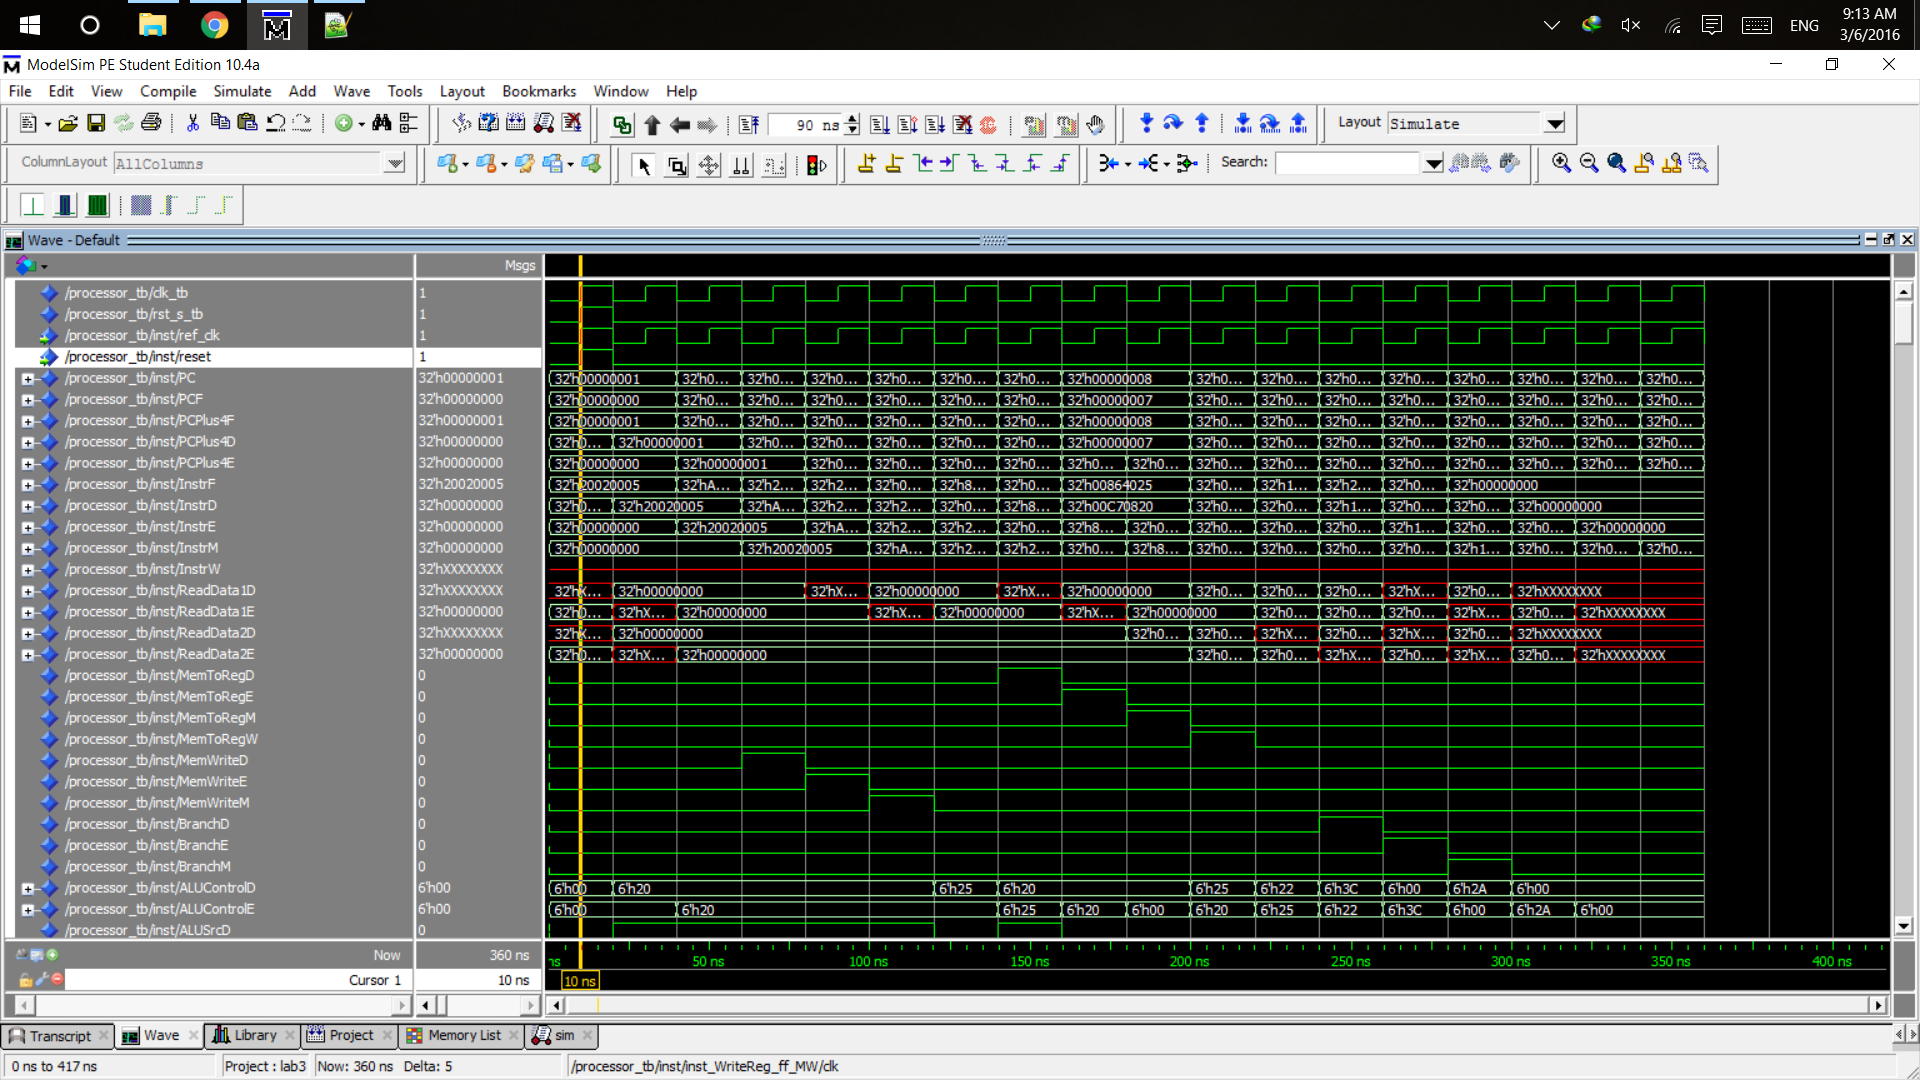
\includegraphics[width=150mm]{reset.png}
	\label{fig:reset}
\end{figure}
\pagebreak
ADDI $2 $zero 5
\begin{figure}[H]
	\centering
		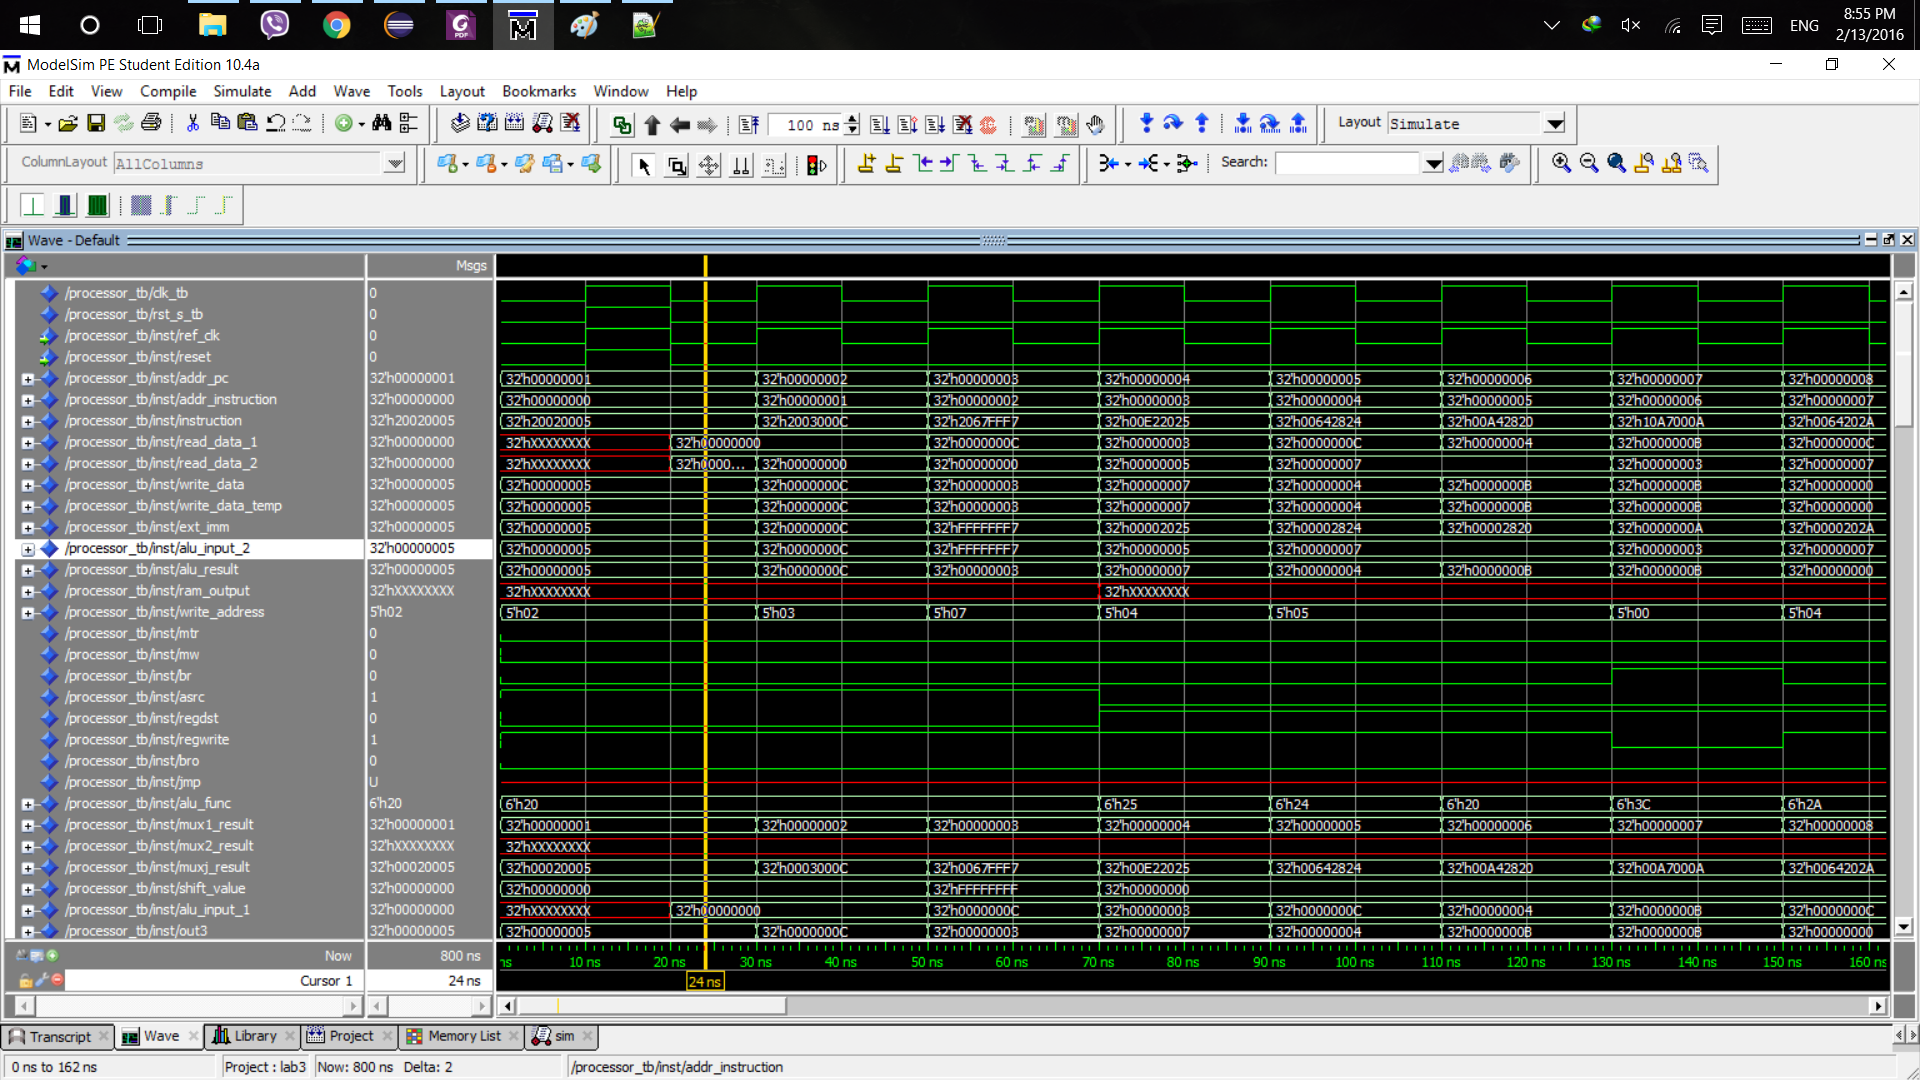
\includegraphics[width=150mm]{0.png}
	\label{fig:0}
\end{figure}

ADDI $3 $zero 12
\begin{figure}[H]
	\centering
		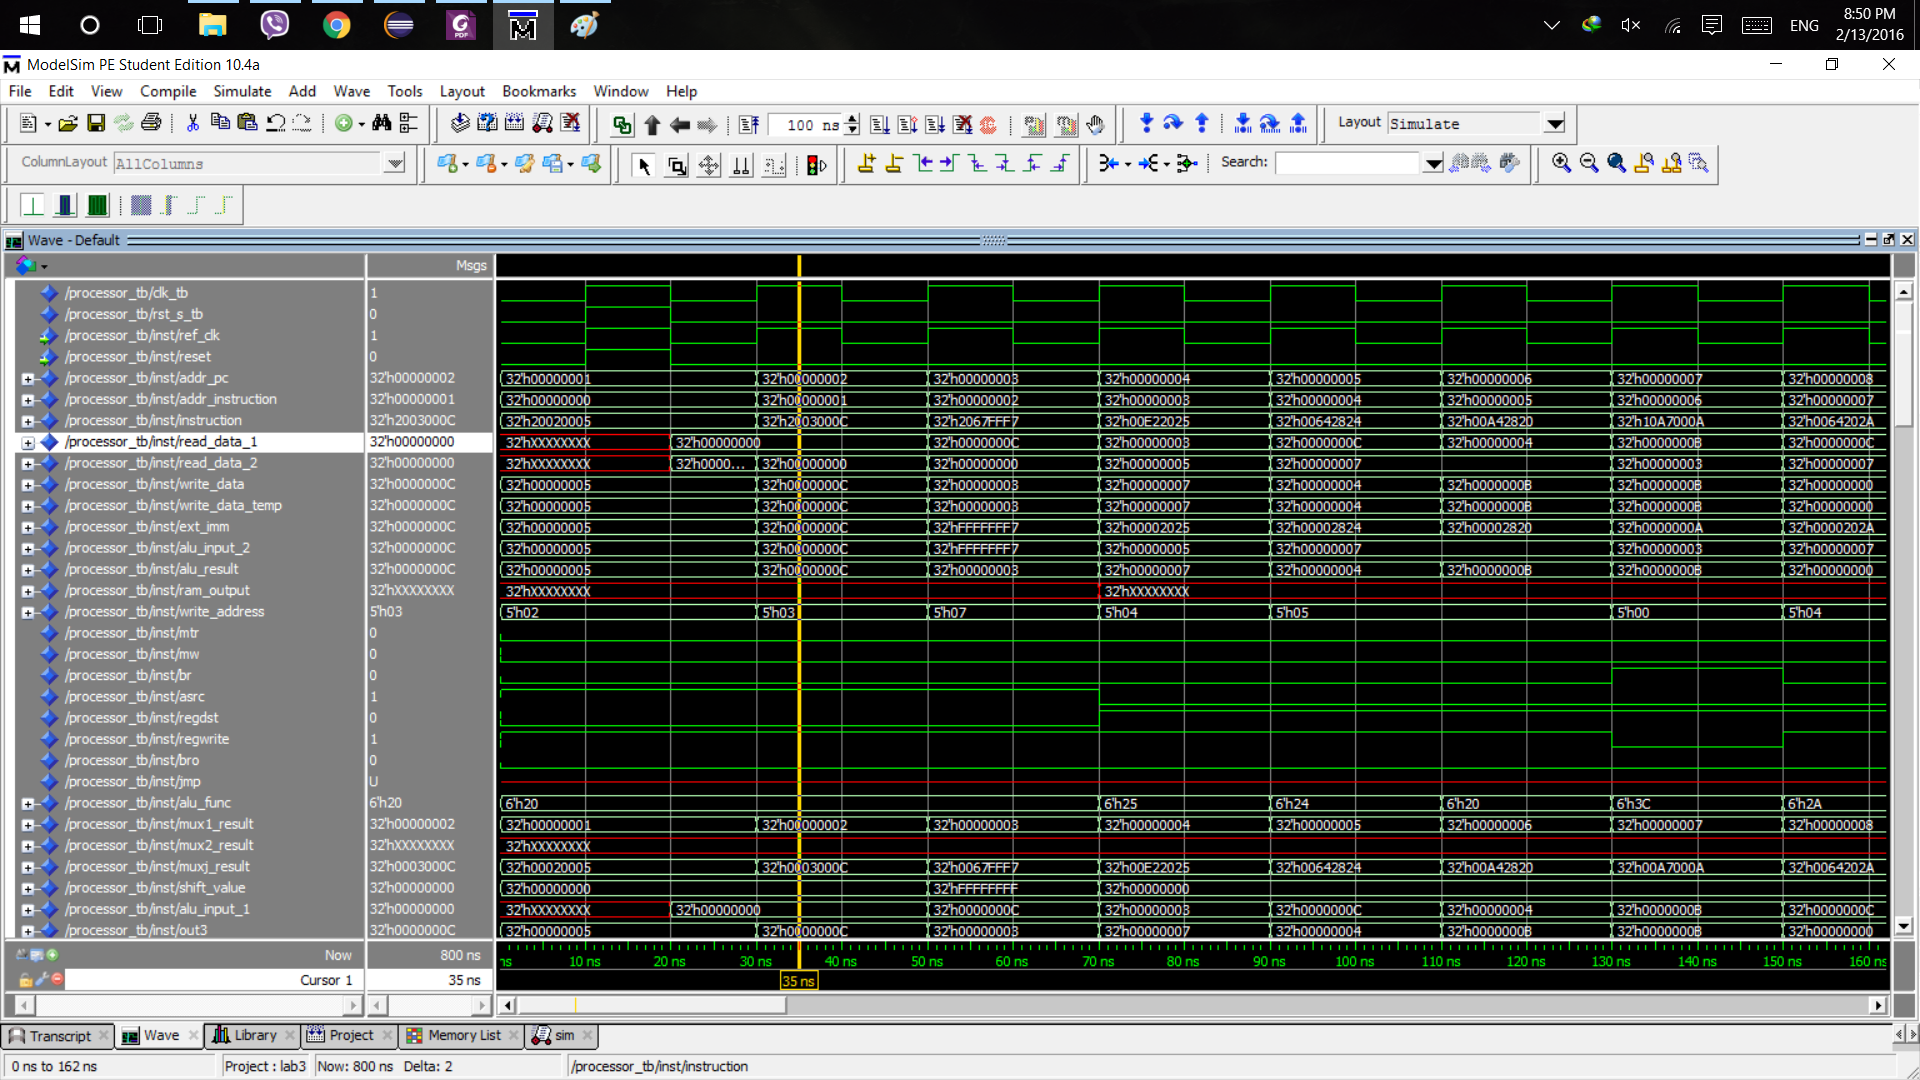
\includegraphics[width=150mm]{1.png}
	\label{fig:tests}
\end{figure}
\pagebreak
ADDI $7 $3 -9	
\begin{figure}[H]
	\centering
		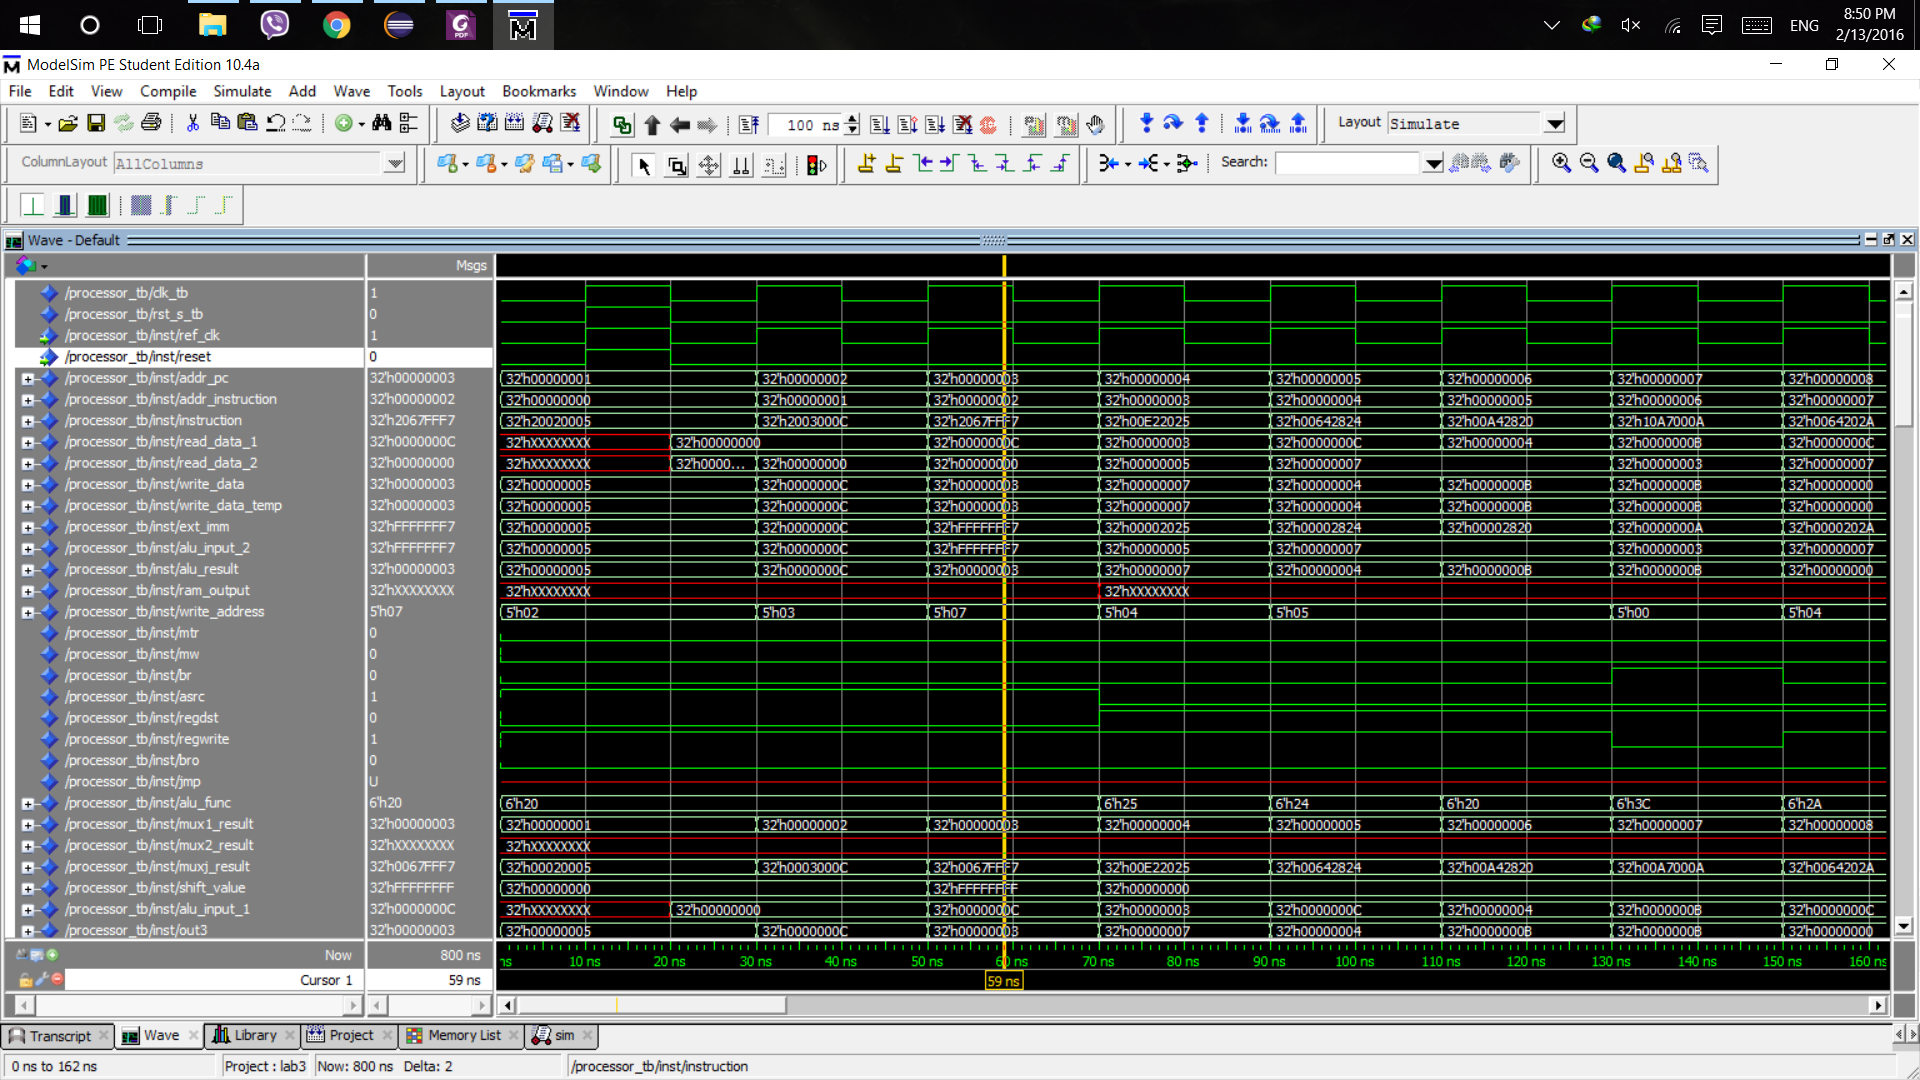
\includegraphics[width=150mm]{2.png}
	\label{fig:tests}
\end{figure}

OR    \$4 \$7 \$2		
\begin{figure}[H]
	\centering
		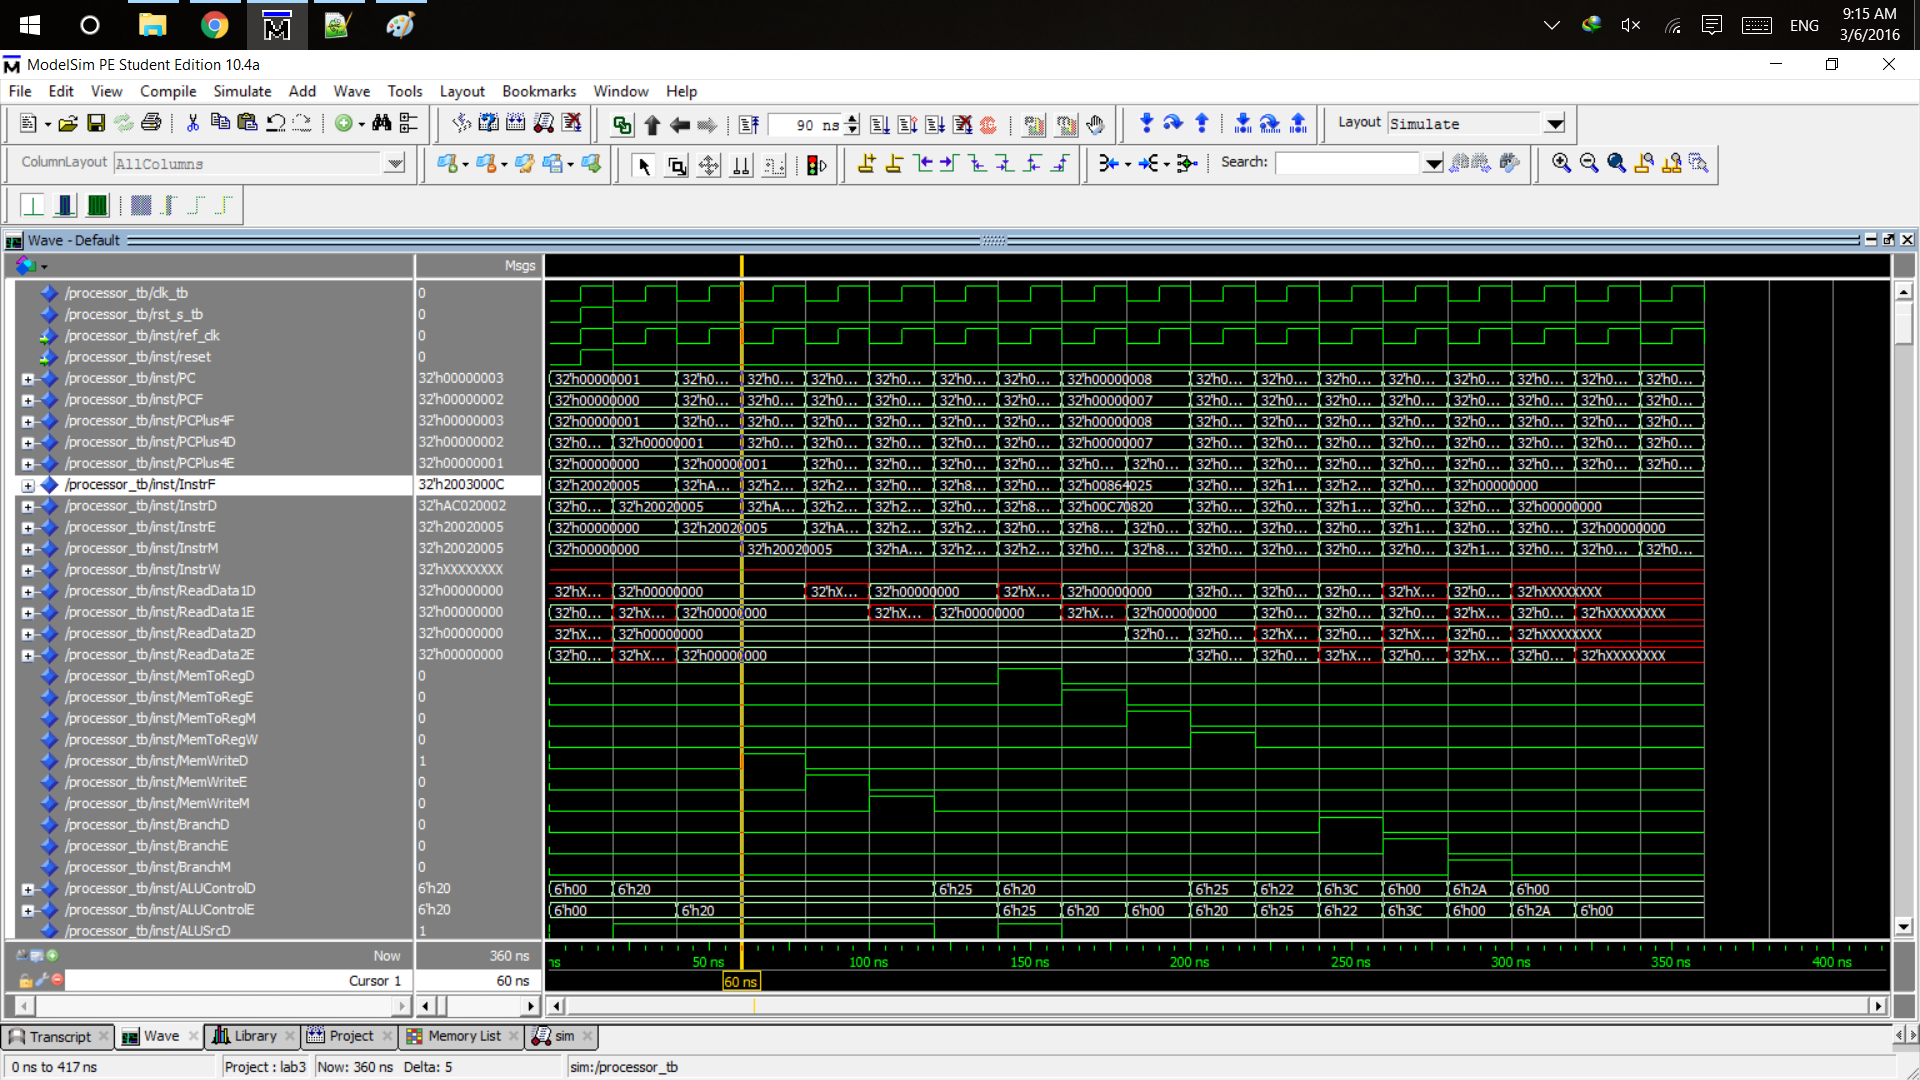
\includegraphics[width=150mm]{3.png}
	\label{fig:tests}
\end{figure}
\pagebreak
AND \$5 \$3 \$4		
\begin{figure}[H]
	\centering
		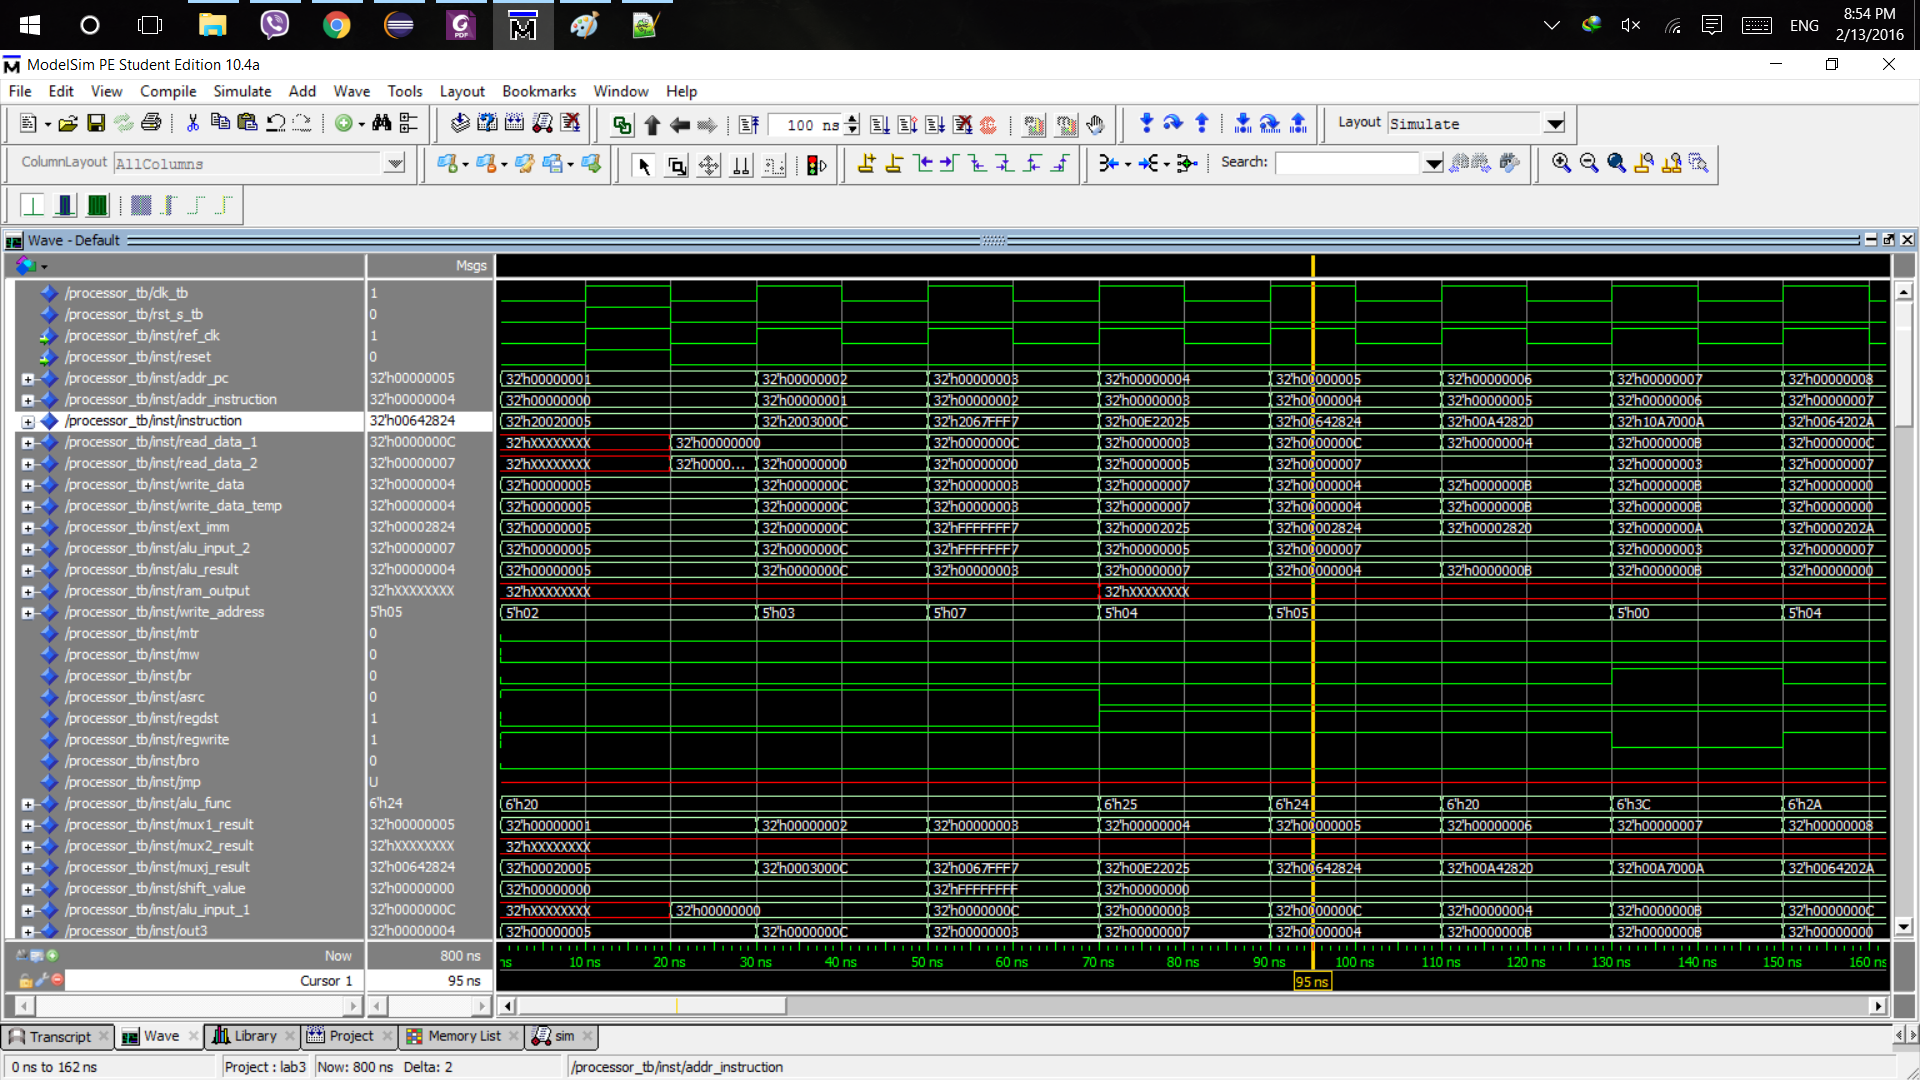
\includegraphics[width=150mm]{4.png}
	\label{fig:tests}
\end{figure}

ADD \$5 \$5 \$4		
\begin{figure}[H]
	\centering
		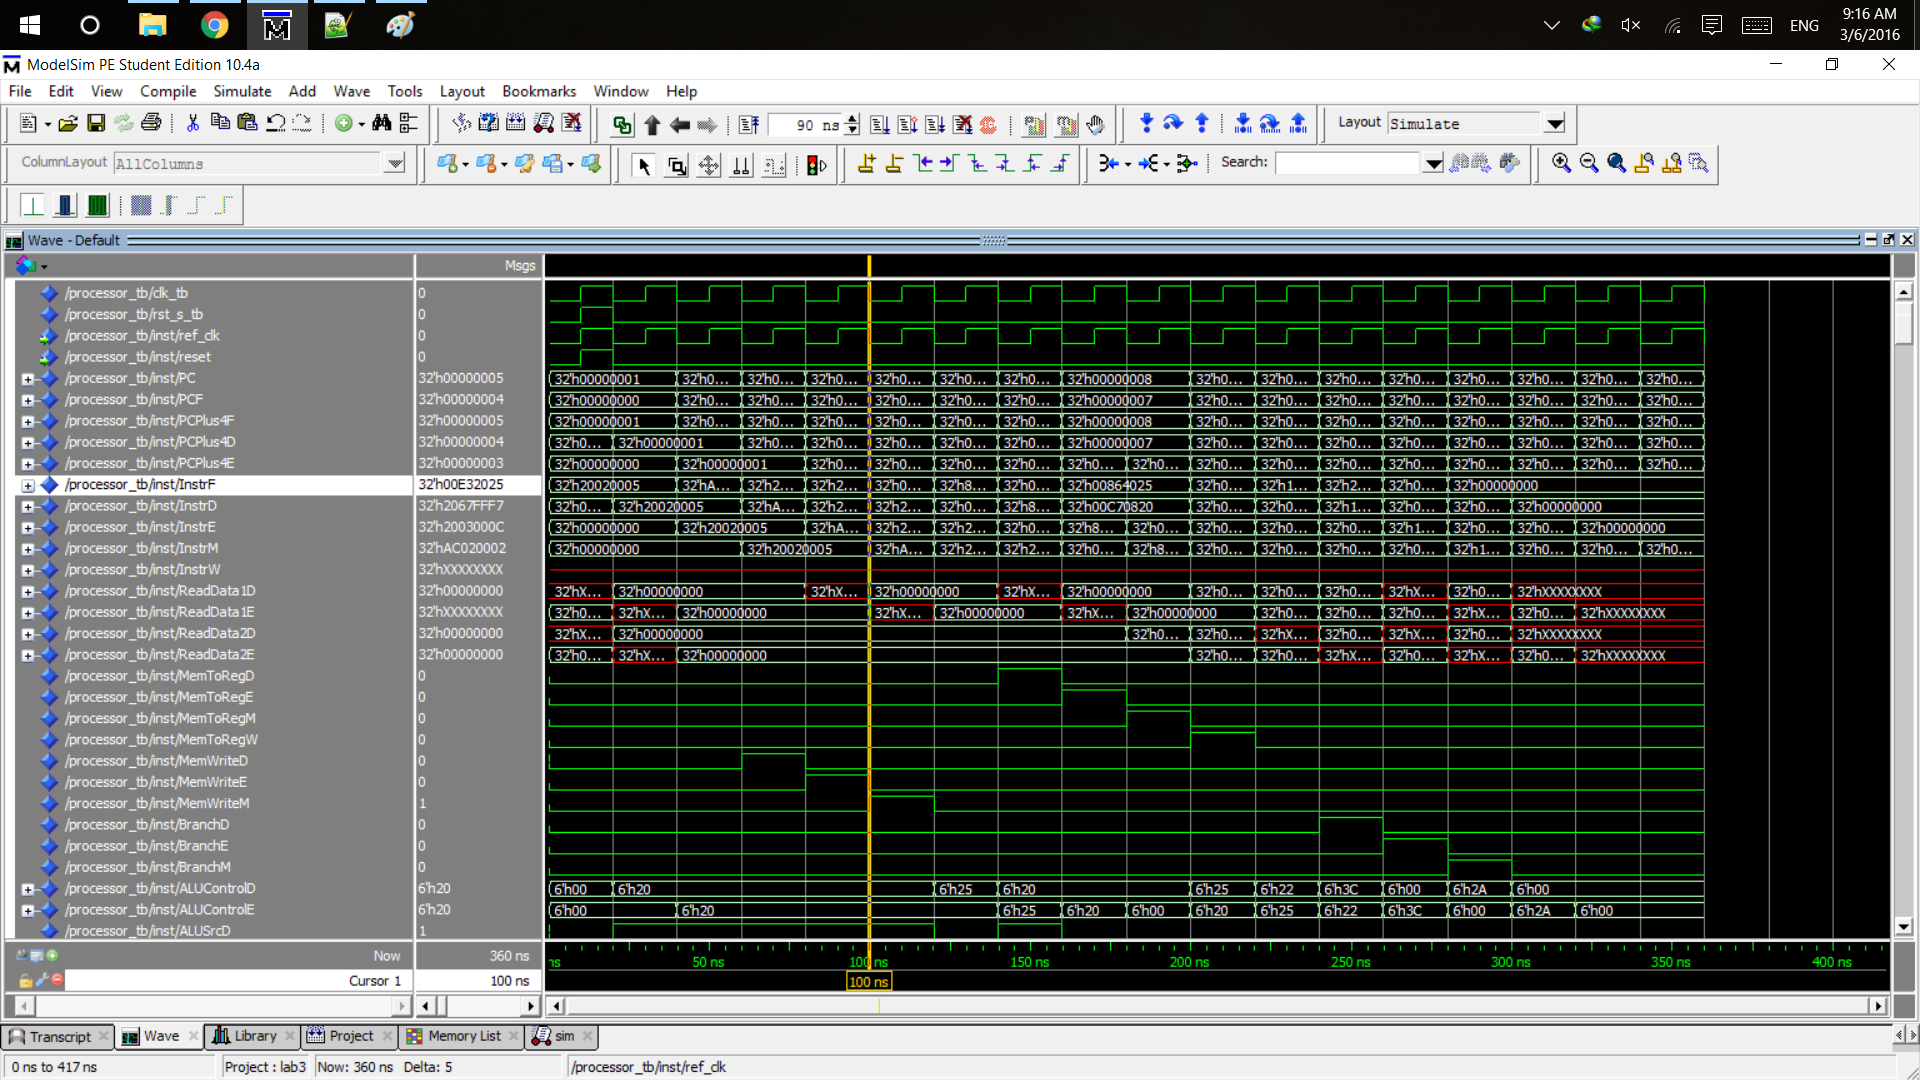
\includegraphics[width=150mm]{5.png}
	\label{fig:tests}
\end{figure}
\pagebreak
BEQ \$5 \$7 10		
\begin{figure}[H]
	\centering
		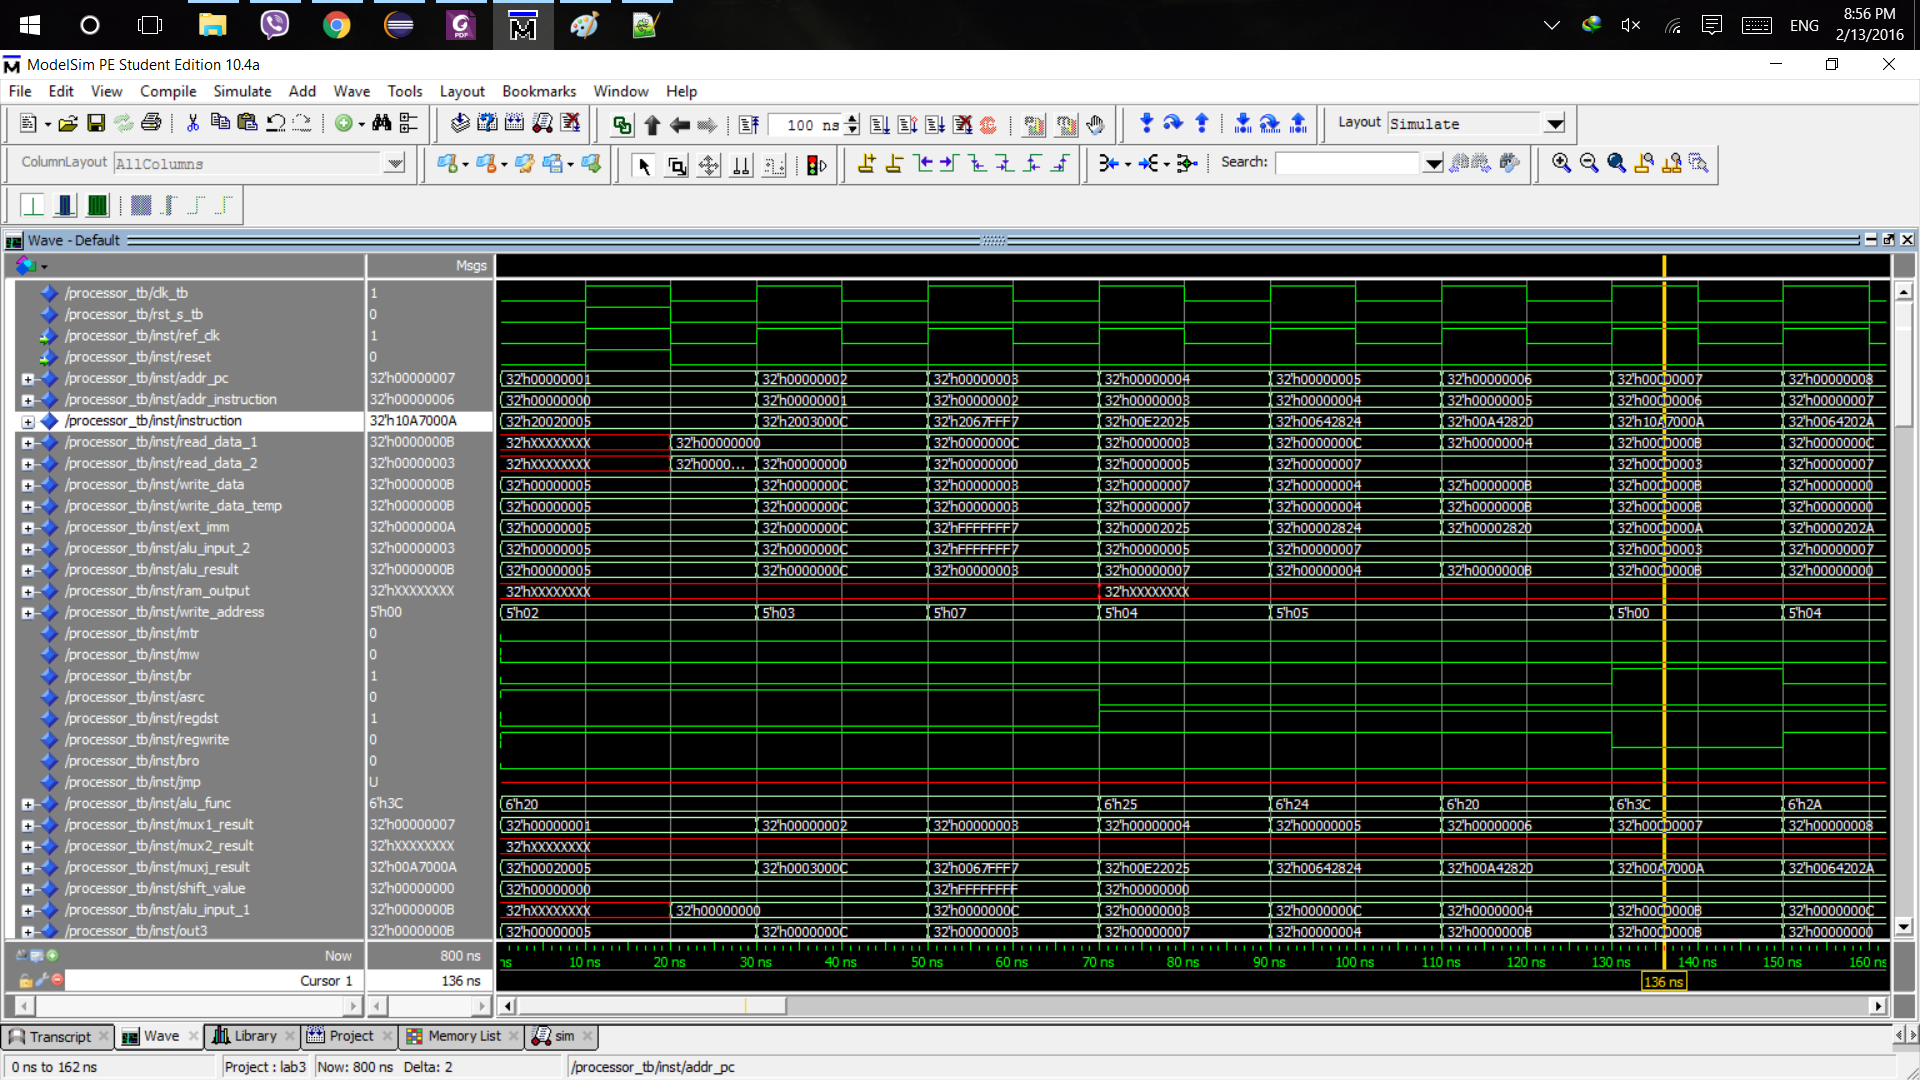
\includegraphics[width=150mm]{6.png}
	\label{fig:tests}
\end{figure}

SLT \$4 \$3 \$4	
\begin{figure}[H]
	\centering
		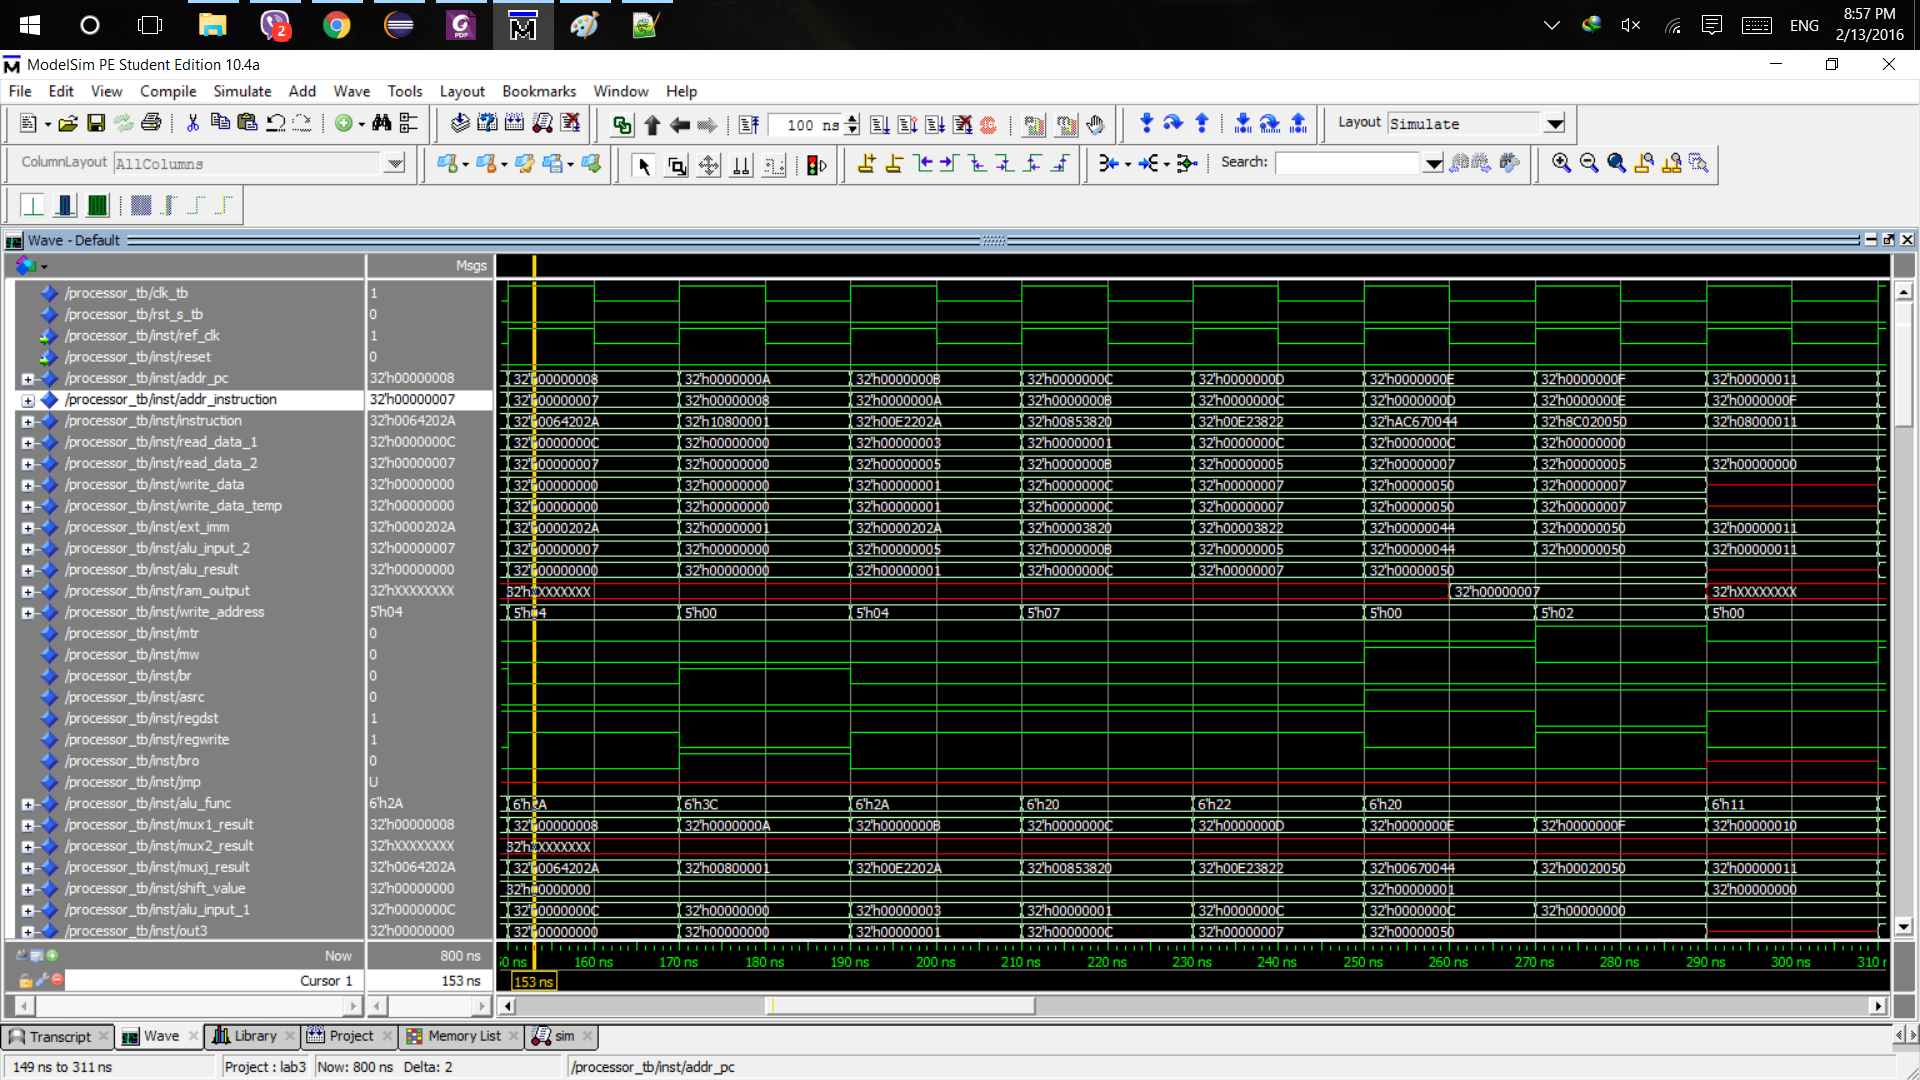
\includegraphics[width=150mm]{7.png}
	\label{fig:tests}
\end{figure}
\pagebreak
BEQ \$4 \$zero 1		
\begin{figure}[H]
	\centering
		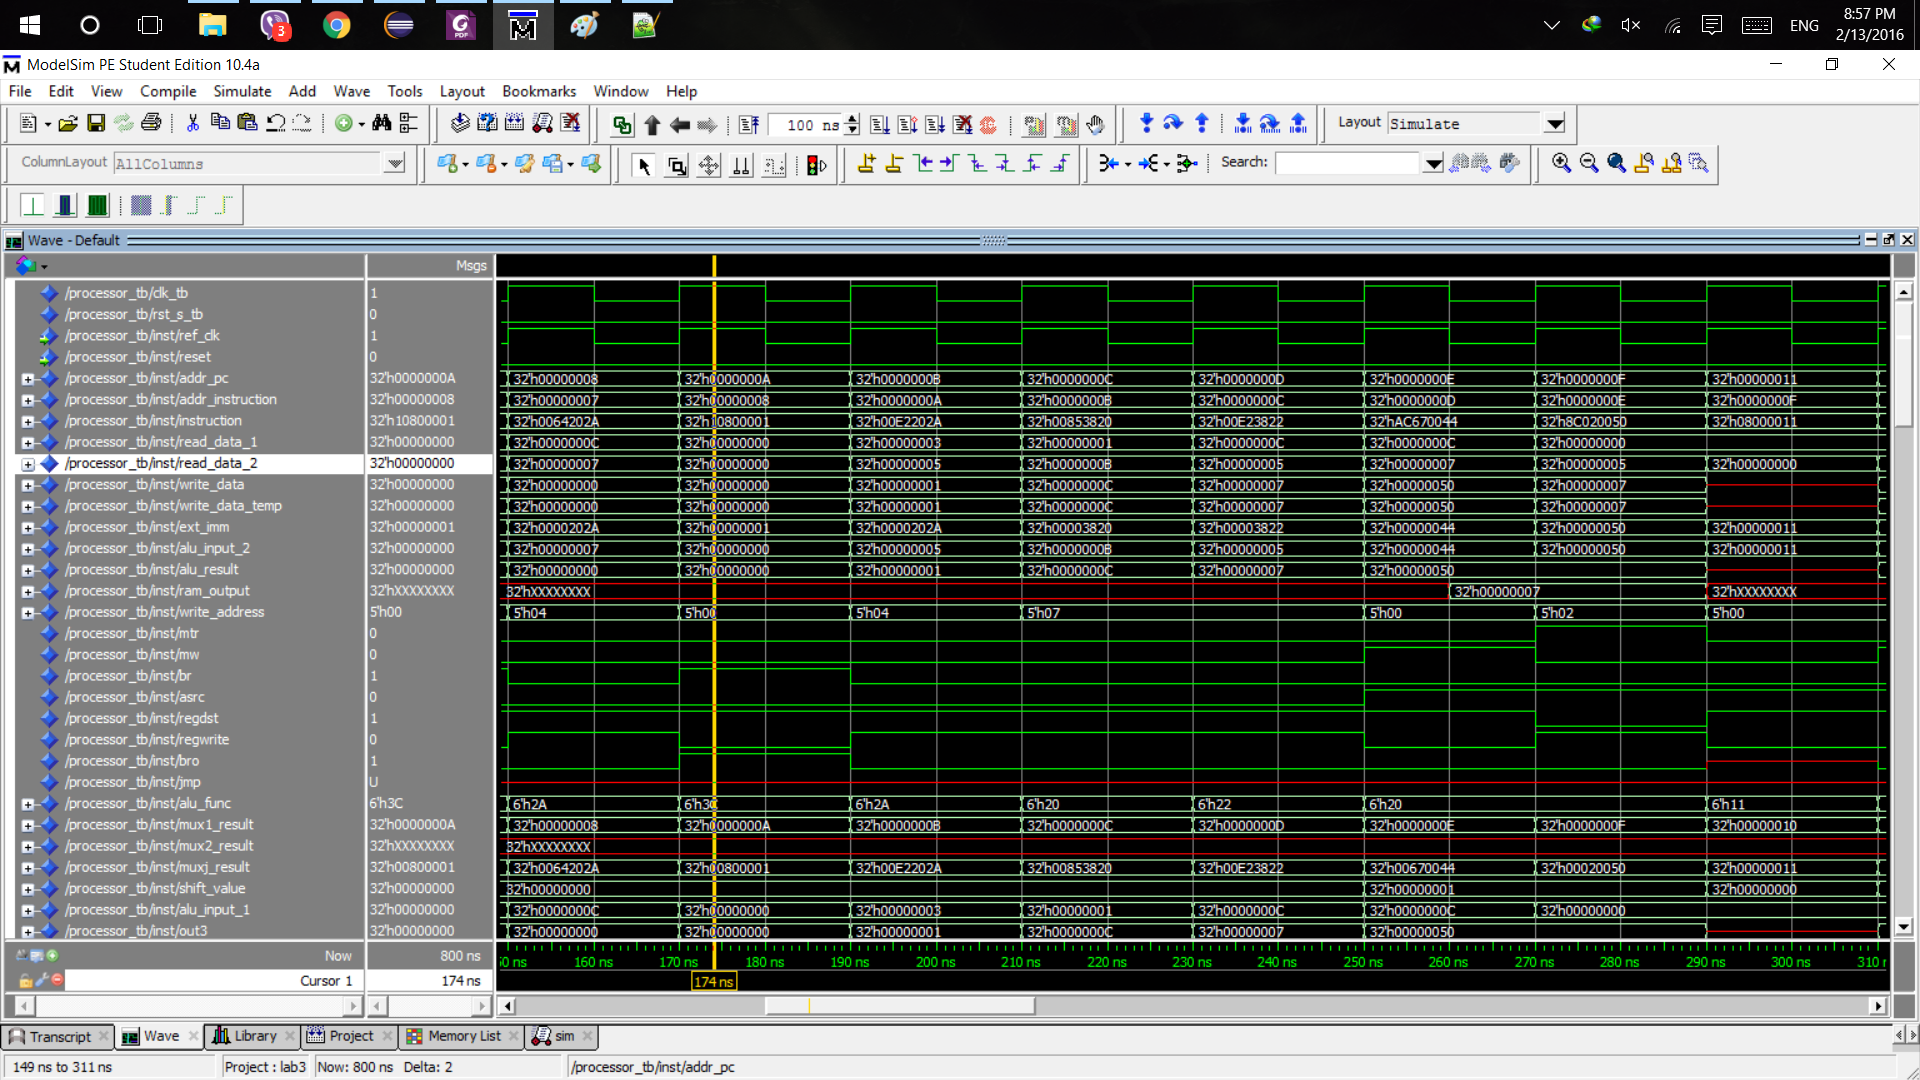
\includegraphics[width=150mm]{8.png}
	\label{fig:tests}
\end{figure}

ADDI \$5 \$zero 0		\\
This instruction does not execute due to the branch. 
\\
\pagebreak
SLT \$4 \$7 \$2			
\begin{figure}[H]
	\centering
		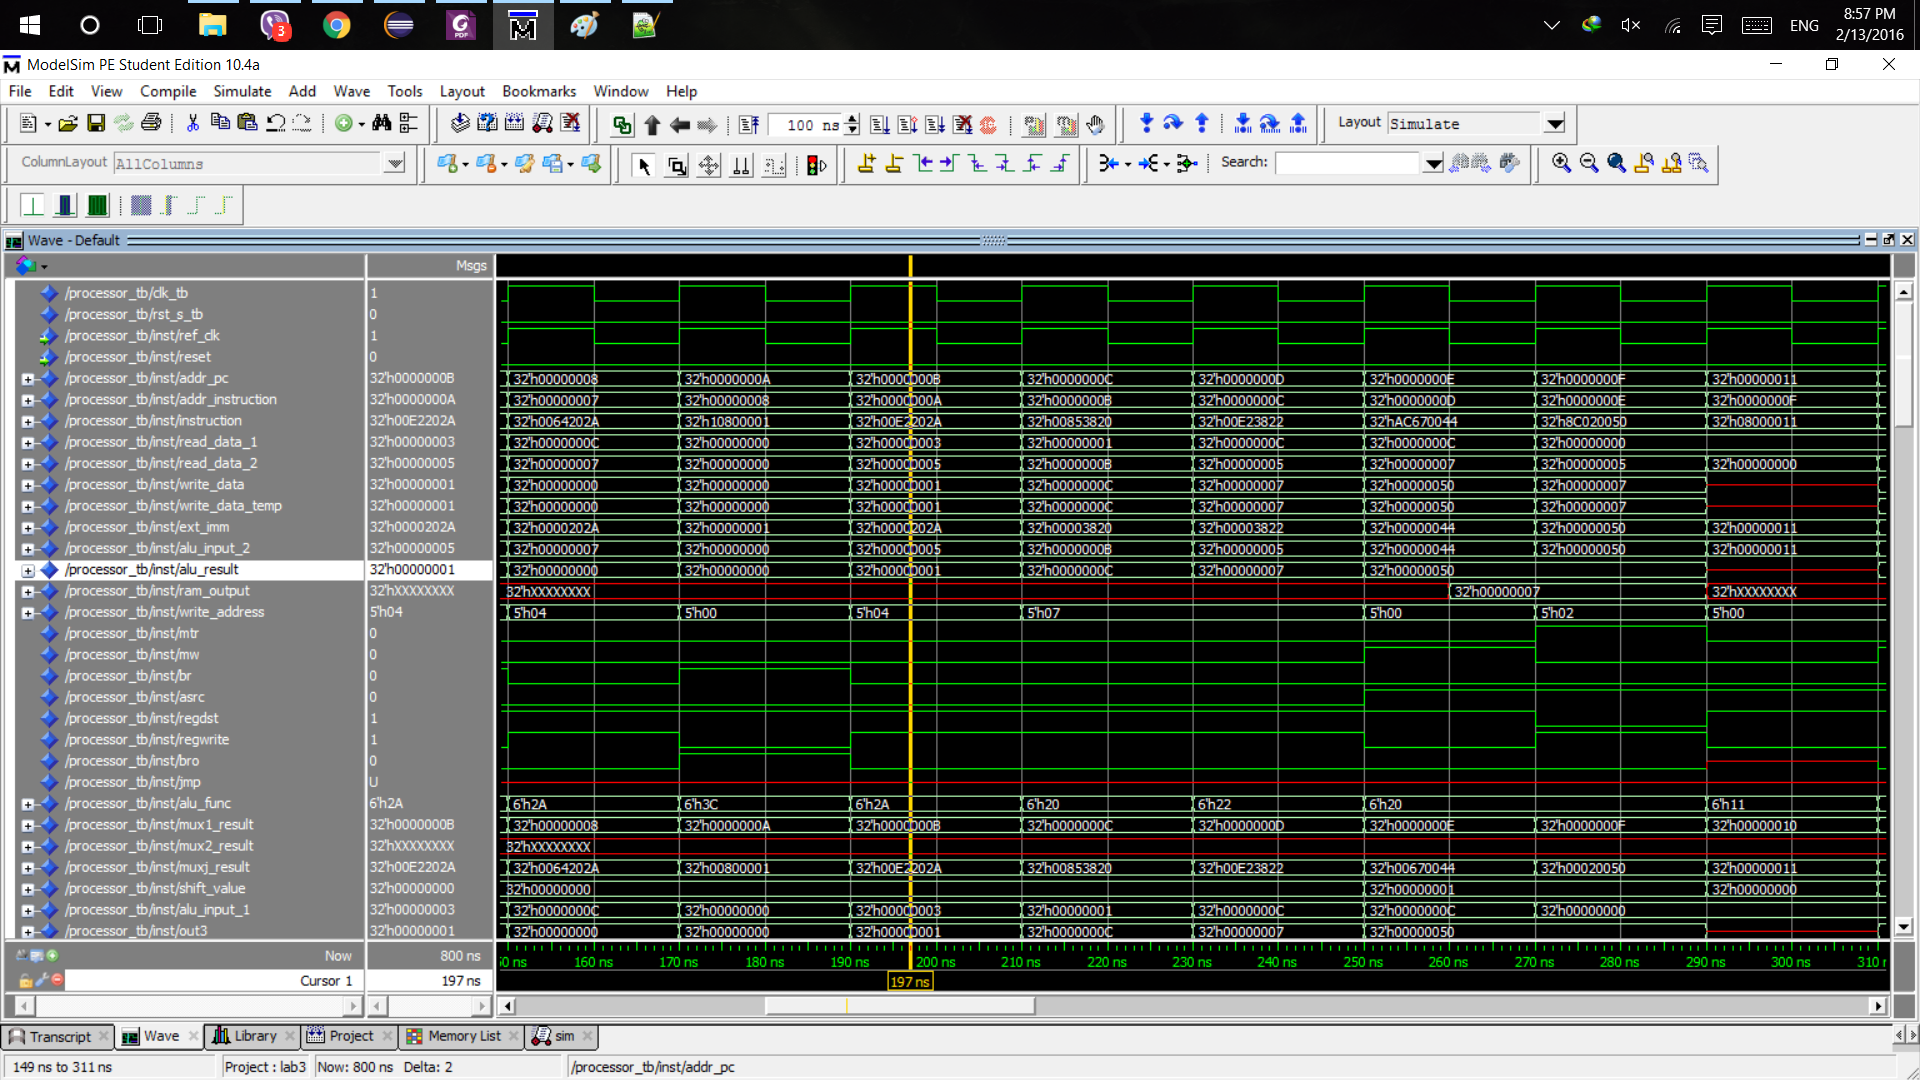
\includegraphics[width=150mm]{10.png}
	\label{fig:tests}
\end{figure}

ADD \$7 \$4 \$5		
\begin{figure}[H]
	\centering
		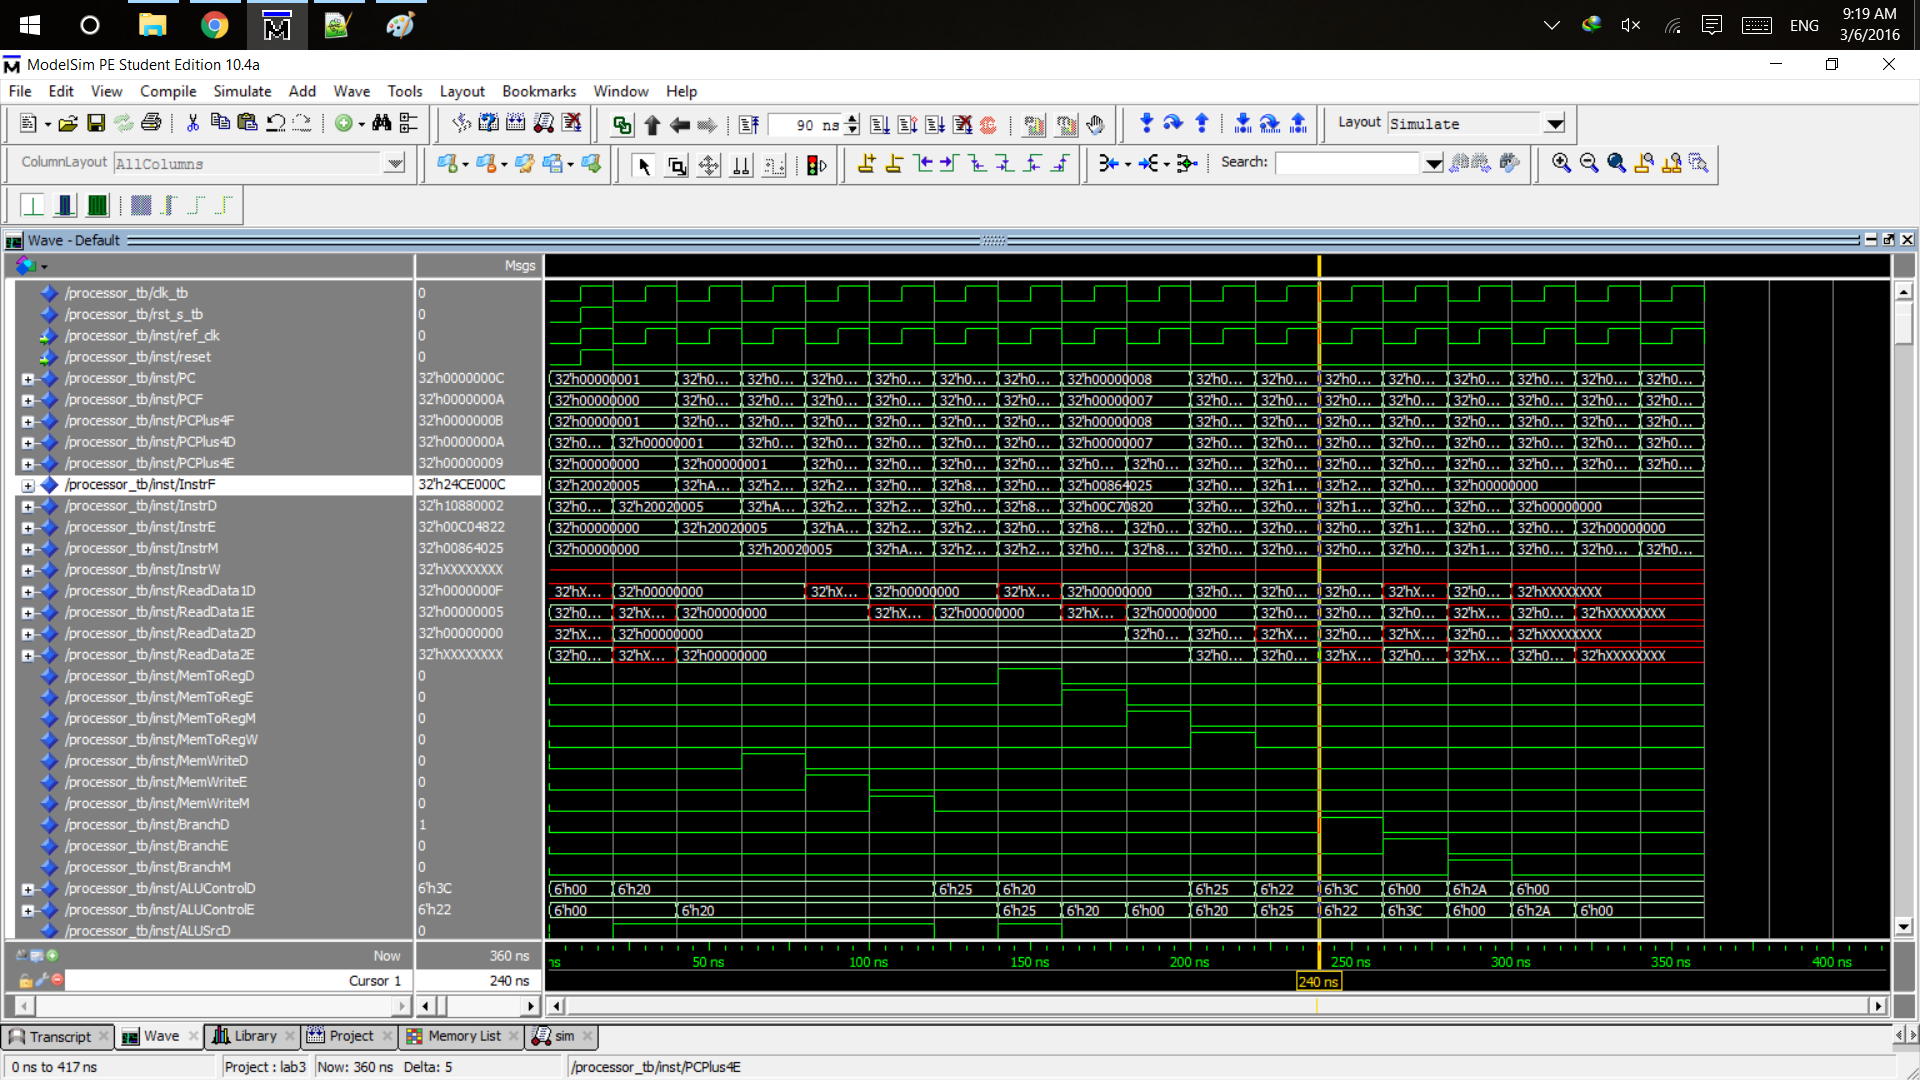
\includegraphics[width=150mm]{11.png}
	\label{fig:tests}
\end{figure}
\pagebreak
SUB \$7 \$7 \$2		
\begin{figure}[H]
	\centering
		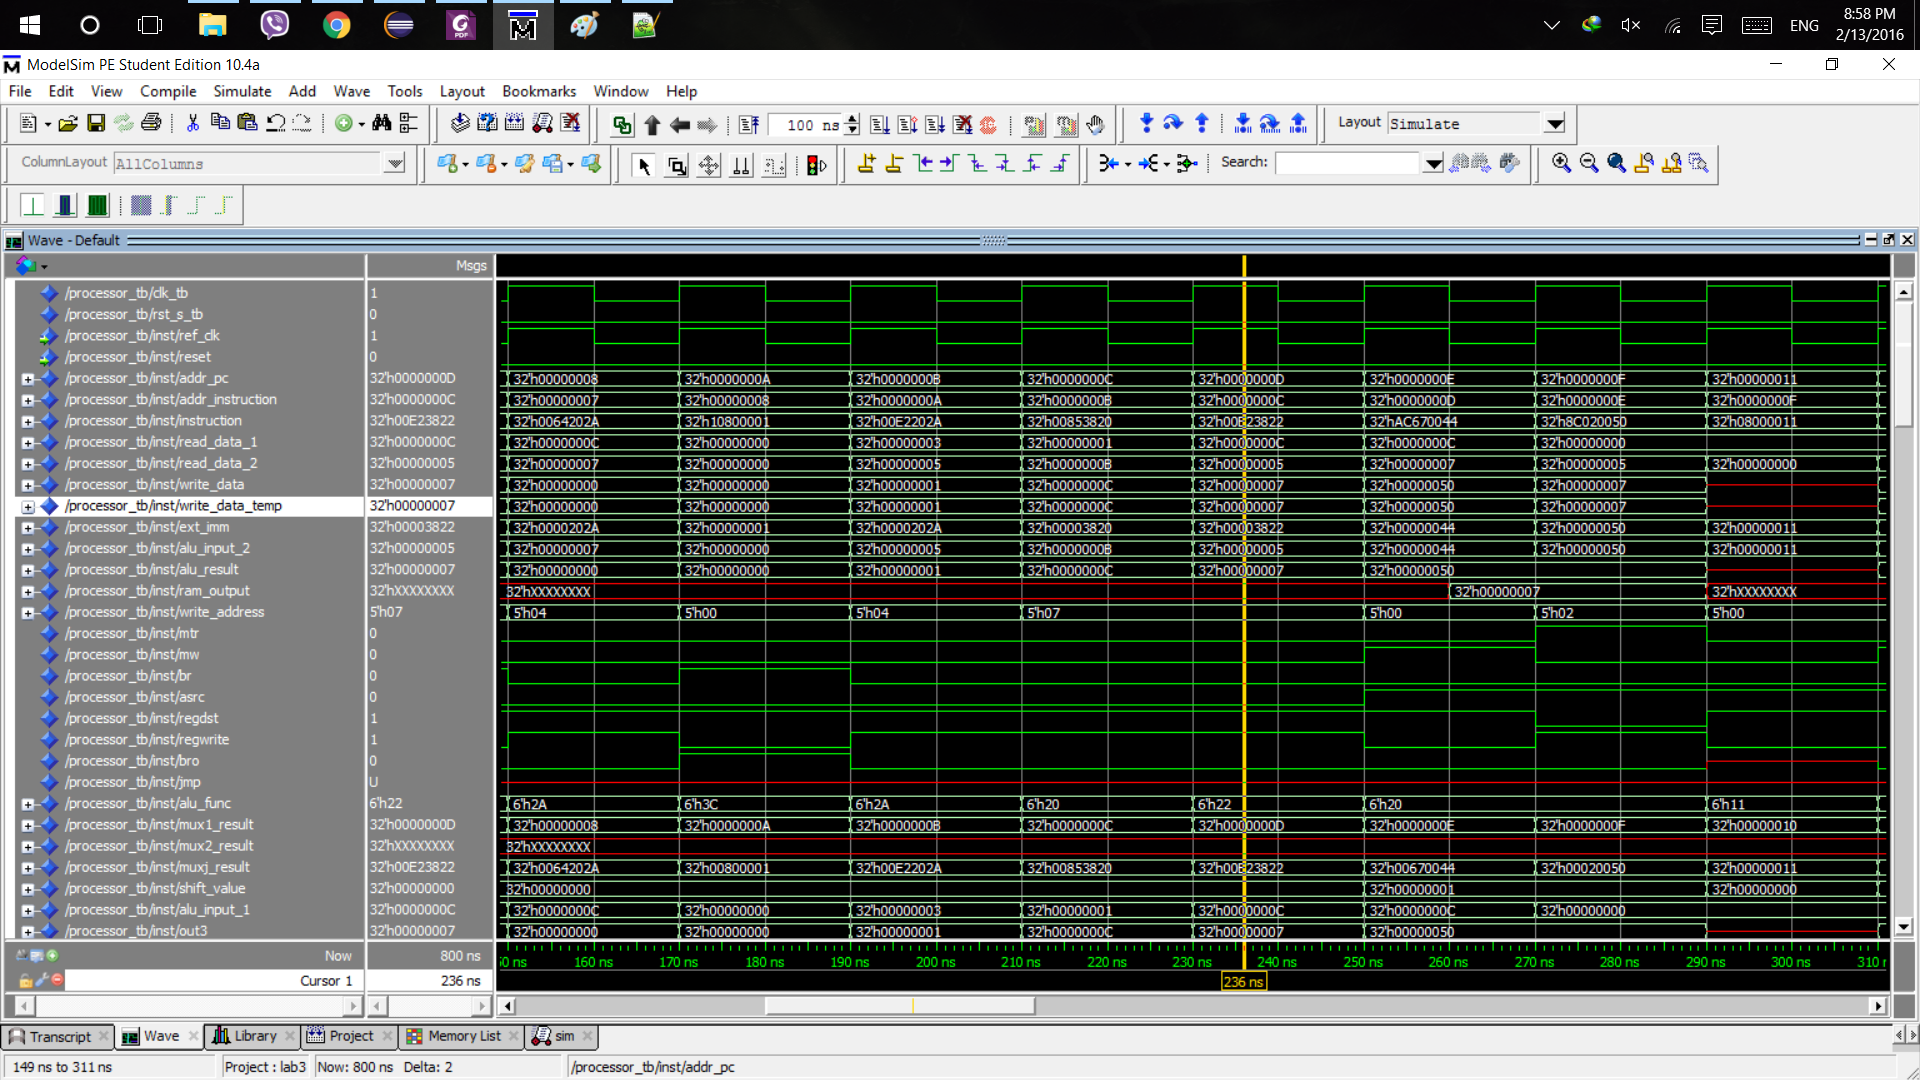
\includegraphics[width=150mm]{12.png}
	\label{fig:tests}
\end{figure}

SW \$7 68(\$3)		
\begin{figure}[H]
	\centering
		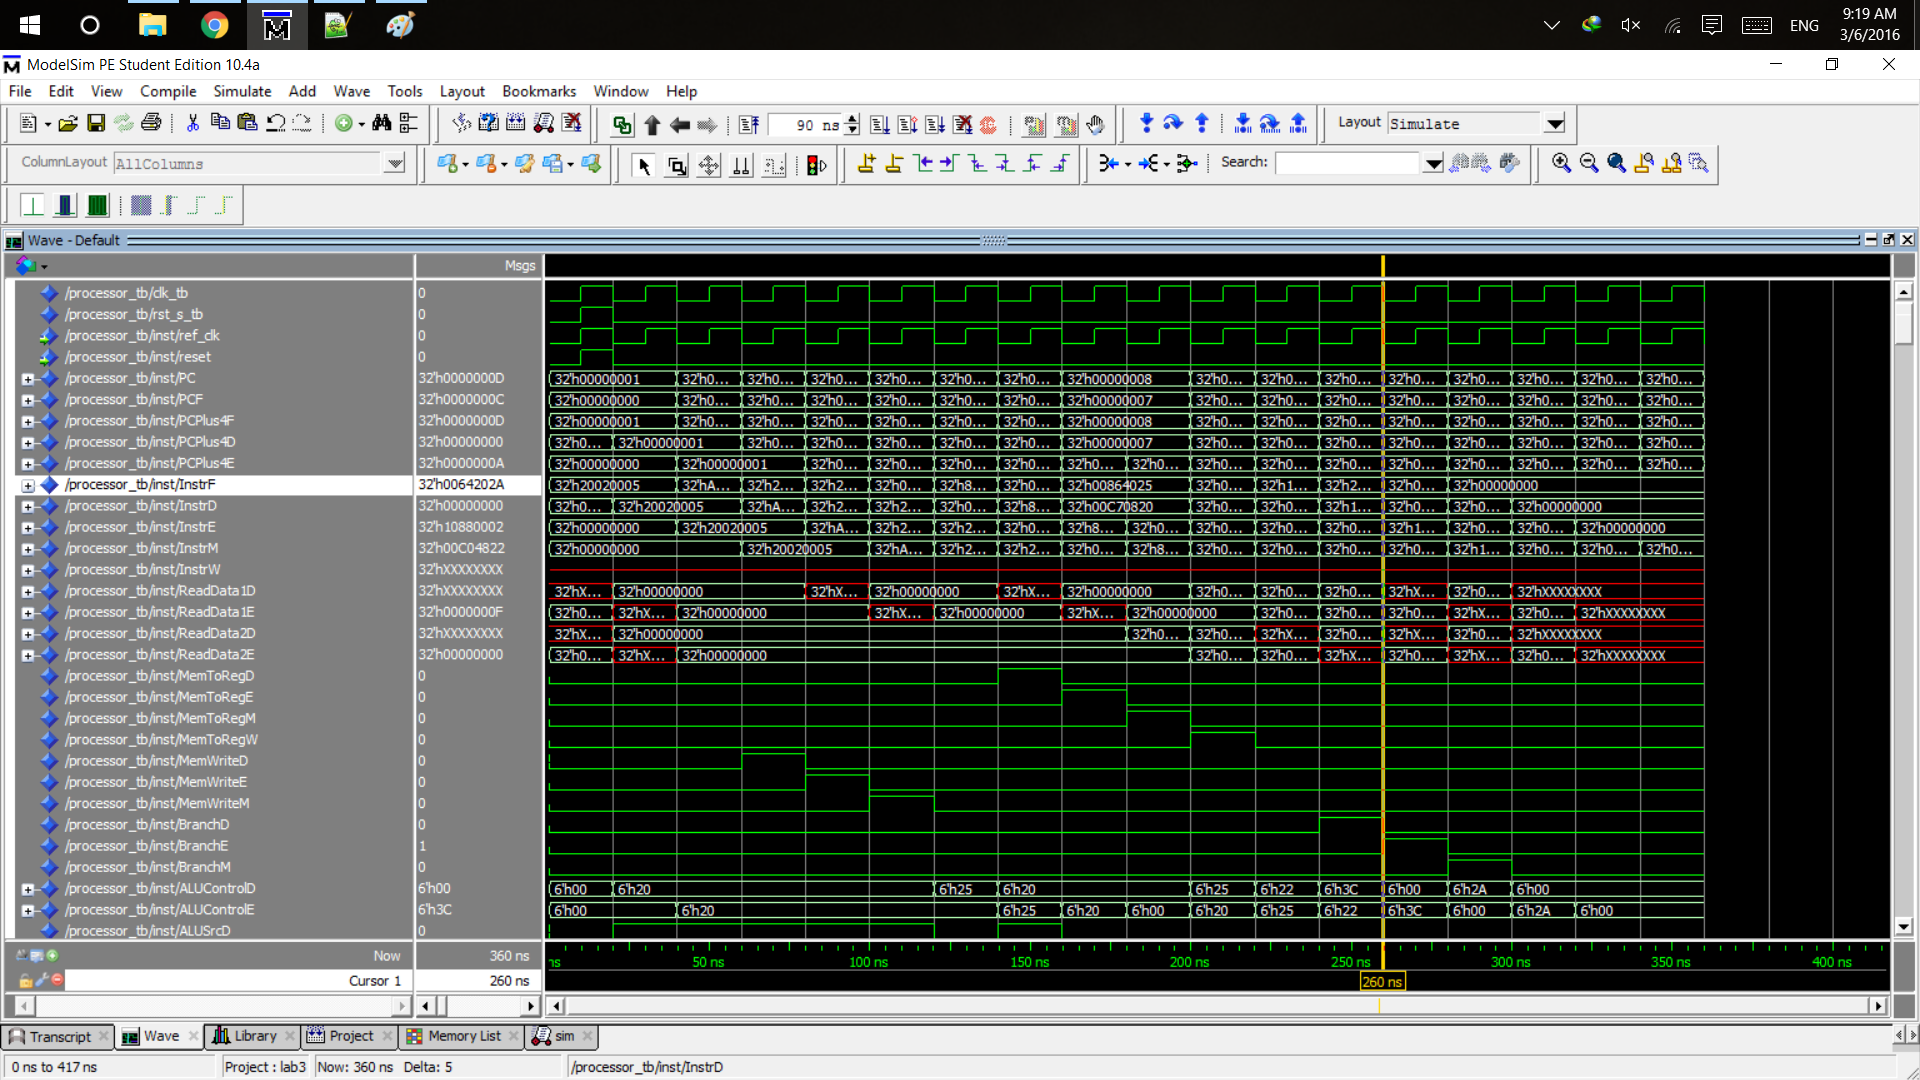
\includegraphics[width=150mm]{13.png}
	\label{fig:tests}
\end{figure}
\pagebreak
LW \$2 80(\$zero)
\begin{figure}[H]
	\centering
		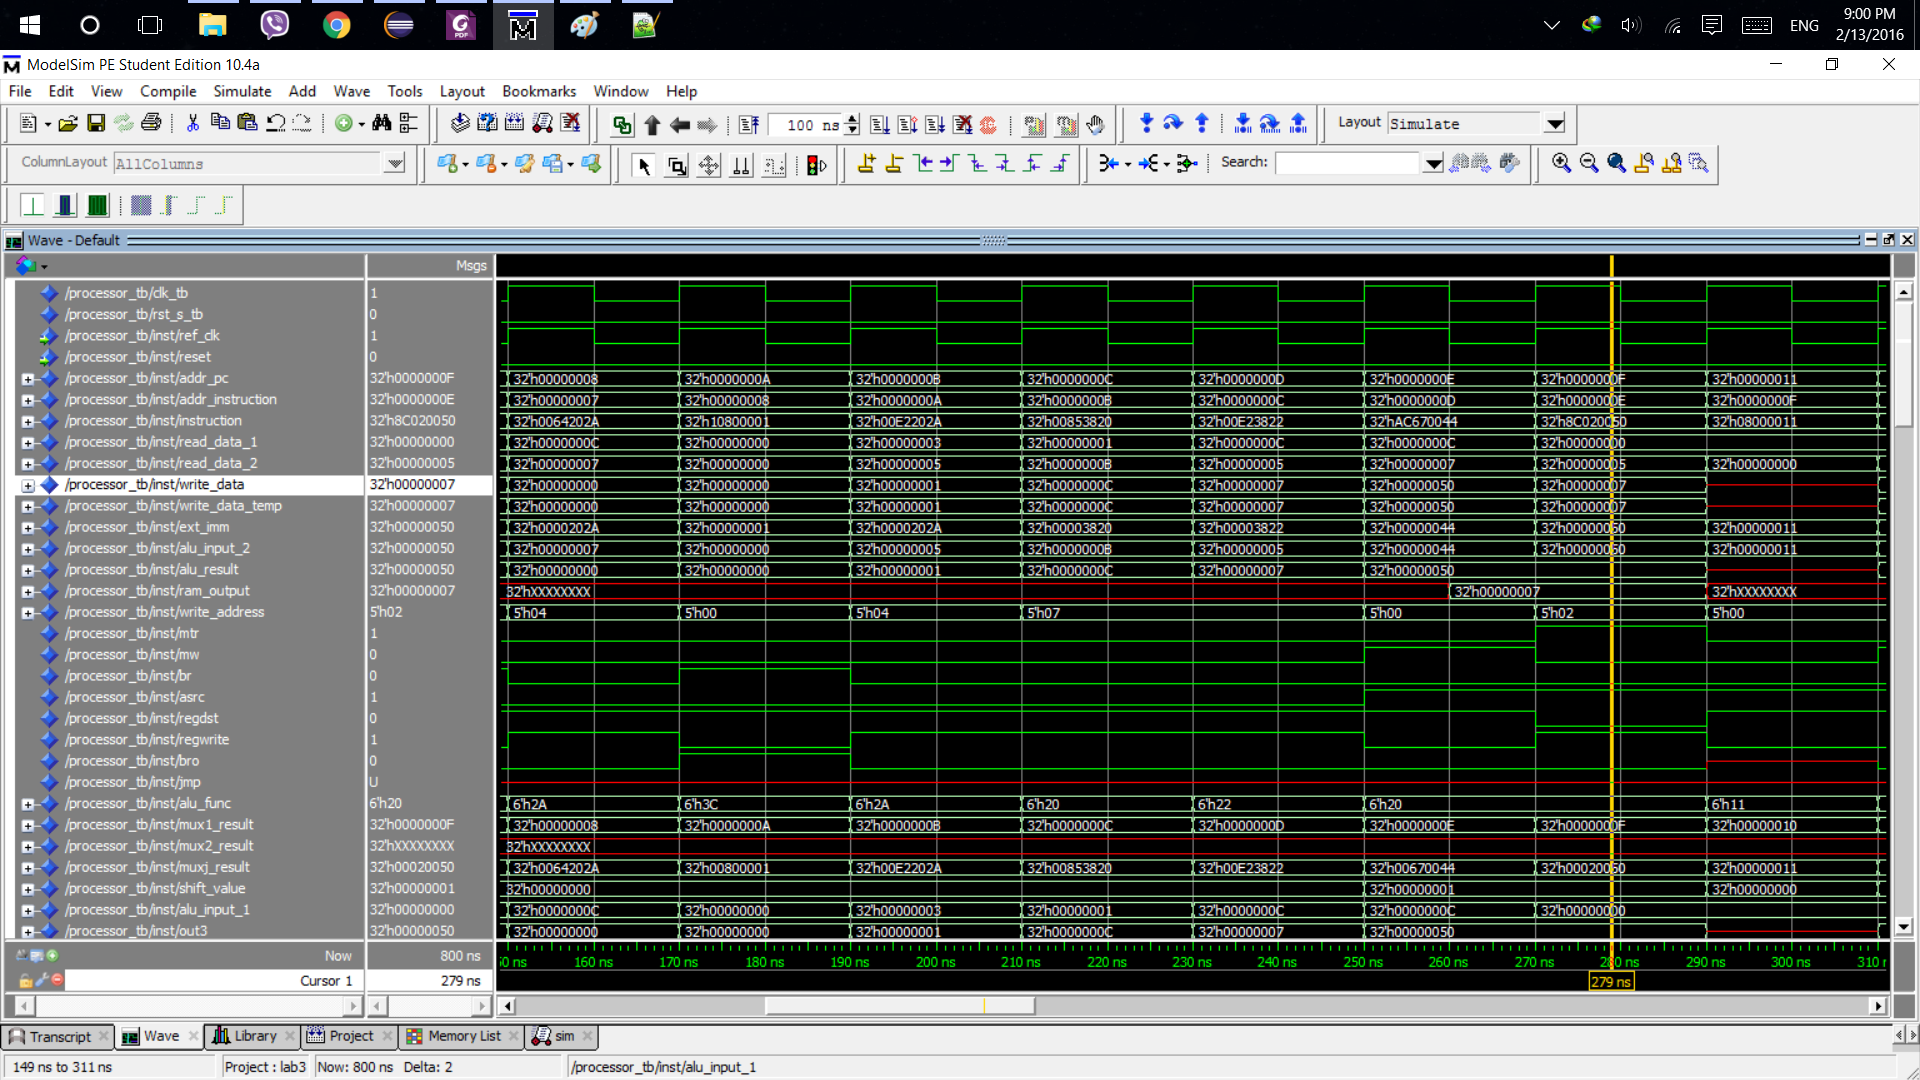
\includegraphics[width=150mm]{14.png}
	\label{fig:tests}
\end{figure}

J 17										
\begin{figure}[H]
	\centering
		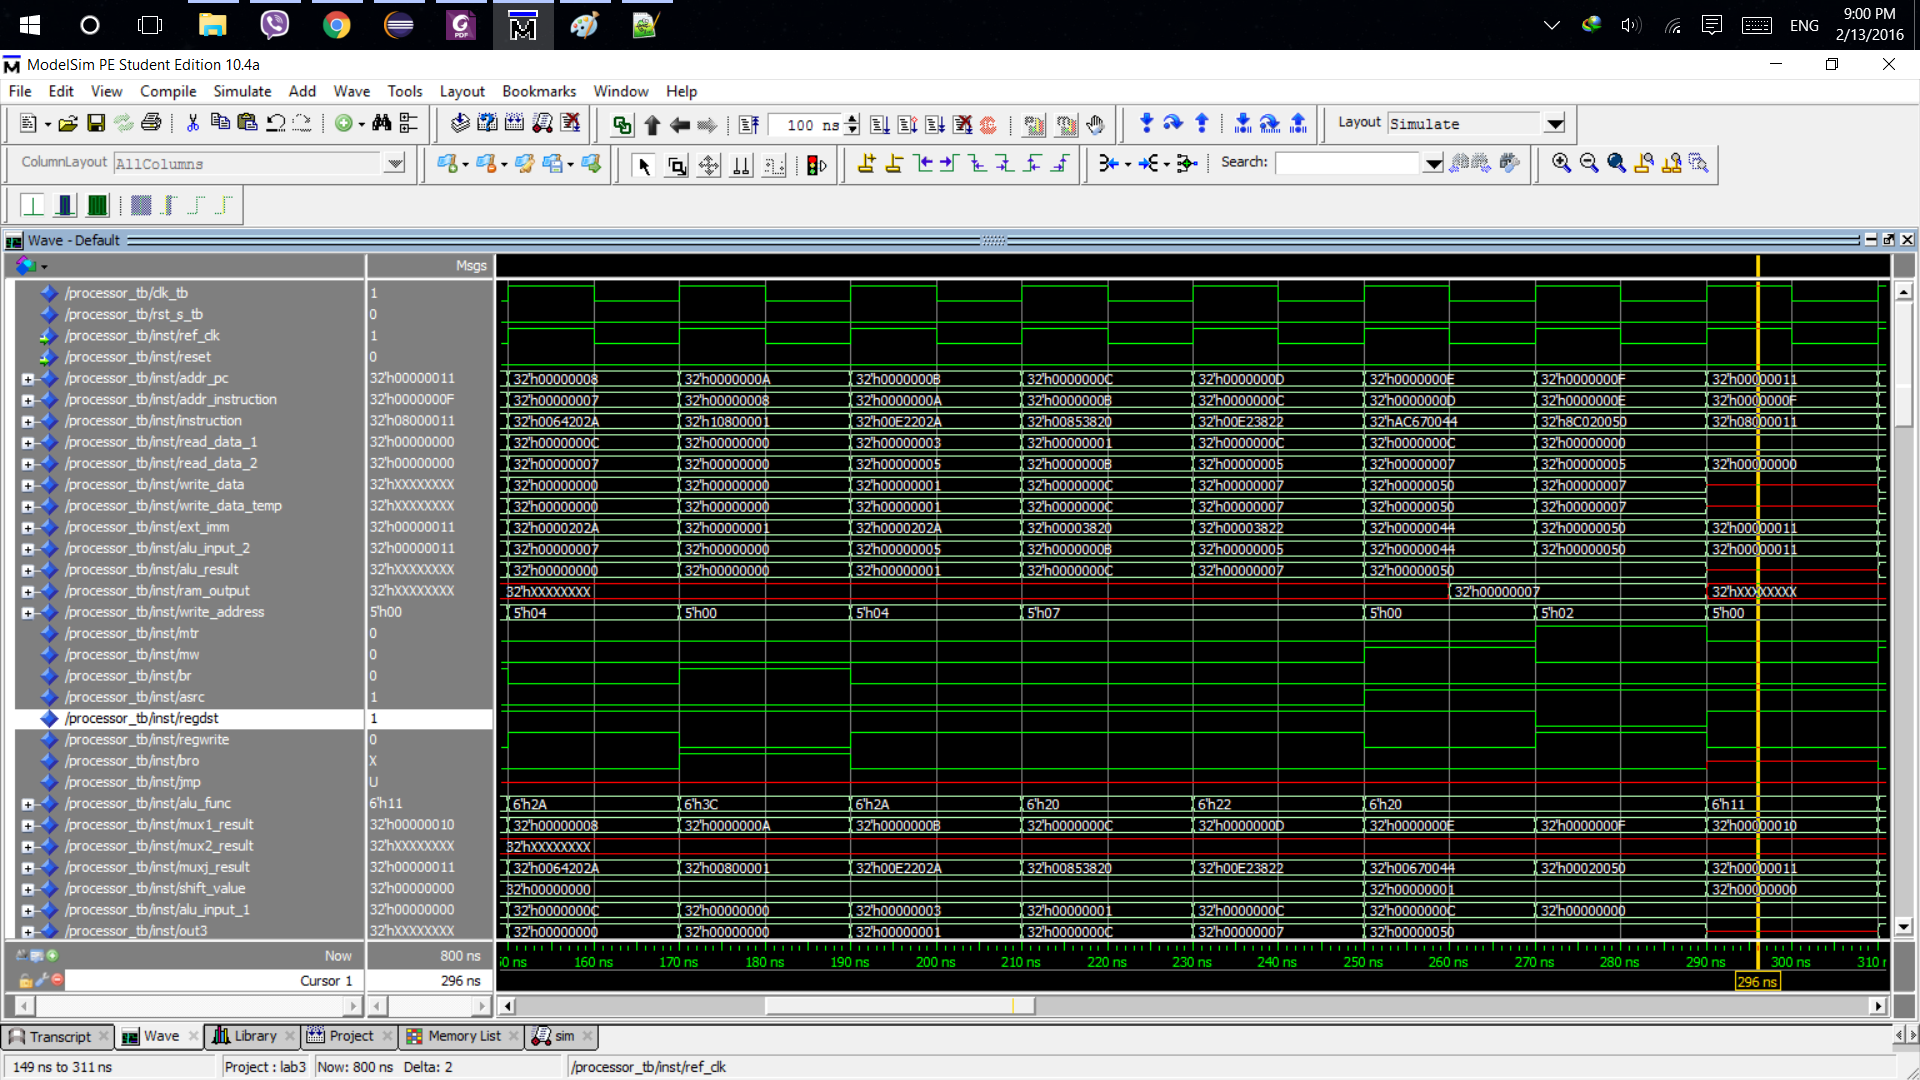
\includegraphics[width=150mm]{15.png}
	\label{fig:tests}
\end{figure}
\pagebreak
ADDI \$2 \$zero 1 \\
This instruction does not execute due to jump.
\\

SW \$2 84(\$zero)
\begin{figure}[H]
	\centering
		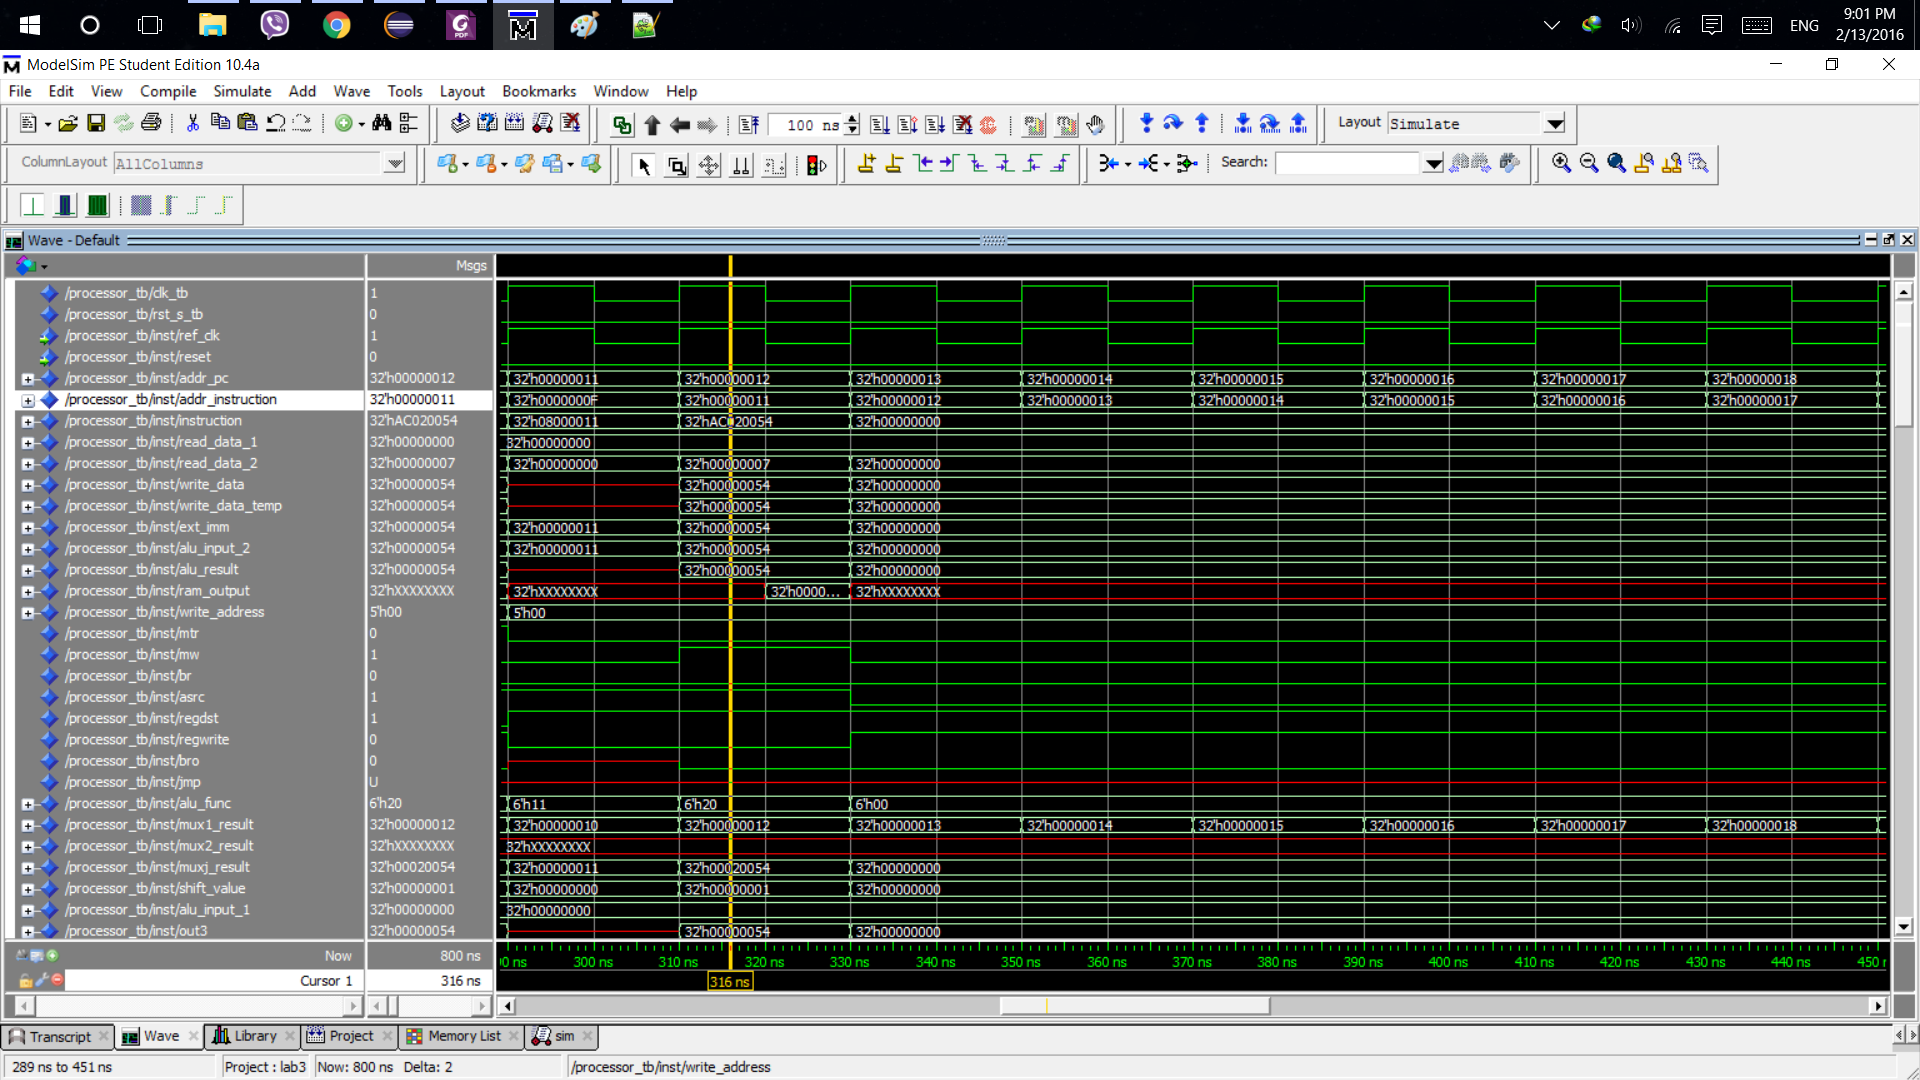
\includegraphics[width=150mm]{17.png}
	\label{fig:tests}
\end{figure}

\pagebreak

%----------------------------------------------------------------------------------------
% SYNTHESIS
%----------------------------------------------------------------------------------------

\section{Synthesis}
For the synthesis we received the following results:
\\
Total area = 1685.002450
\\
Power (flat) = 129.350uW
\\
For the more detailed reports of the synthesis of our design they can be found inside the synth/MIPS/reports folder.
\\
\pagebreak
%----------------------------------------------------------------------------------------
%	CONCLUSION
%----------------------------------------------------------------------------------------

\section{Conclusion}
In the end, our program compiled fully with some warnings here and there (the warnings are shown below). These warnings appear at the third instruction we load, which is the ``ADDI \$7 \$3 -9'' instruction; however, these warnings do not affect the results of the instructions loaded.

\begin{figure}
	\centering
		\includegraphics[width=150mm]{warnings.jpg}
	\label{fig:warnings}
\end{figure}

\end{document}